%% =====================================================================
%%  WaveLink Chat -- Final Project Report
%%  EN2130 Communication Design Project (2026)
%%
%%  Compile with:  pdflatex WaveLink_Final_Report.tex   (run it twice,
%%  so the table of contents, cross-references and title page settle)
%%  Needs the folders  figures/  (screenshots, logo)  and  data/  (plot
%%  data computed with the project's own PHY code) next to this file.
%%  Works on Overleaf (TeX Live 2022 or later) and on TeX Live 2023.
%% =====================================================================
\documentclass[11pt,a4paper,oneside]{report}

%% ---------------------------------------------------------------------
%%  EDIT HERE: team, course and institution details
%% ---------------------------------------------------------------------
\newcommand{\TeamName}{Team WaveLink}
\newcommand{\MemberA}{Member Name 1}  \newcommand{\IndexA}{Index No.}
\newcommand{\MemberB}{Member Name 2}  \newcommand{\IndexB}{Index No.}
\newcommand{\MemberC}{Member Name 3}  \newcommand{\IndexC}{Index No.}
\newcommand{\MemberD}{Member Name 4}  \newcommand{\IndexD}{Index No.}
\newcommand{\CourseCode}{EN2130}
\newcommand{\CourseName}{Communication Design Project}
\newcommand{\Department}{Department of Electronic and Telecommunication Engineering}
\newcommand{\University}{University of Moratuwa, Sri Lanka}
\newcommand{\SubmissionDate}{November 2026}

%% ---------------------------------------------------------------------
%%  Packages
%% ---------------------------------------------------------------------
\usepackage[T1]{fontenc}
\usepackage[utf8]{inputenc}
\usepackage{mathpazo}                 % Palatino text and maths
\usepackage[scaled=0.92]{helvet}      % Helvetica for headings and figures
\usepackage{courier}
\usepackage{textcomp}
\usepackage[a4paper,top=25mm,bottom=25mm,left=27mm,right=25mm,headheight=14pt]{geometry}
\usepackage{microtype}
\usepackage{amsmath,amssymb,mathtools,bm}
\usepackage{graphicx}
\usepackage[table,dvipsnames]{xcolor}
\usepackage{booktabs,tabularx,multirow,array,longtable,colortbl}
\usepackage{siunitx}
\sisetup{group-separator={,},group-minimum-digits=4,detect-all}
\usepackage{enumitem}
\setlist{itemsep=2pt,topsep=4pt,parsep=0pt}
\usepackage{caption}
\usepackage{subcaption}
\usepackage{float}
\usepackage{titlesec}
\usepackage{fancyhdr}
\usepackage{tikz}
\usetikzlibrary{arrows.meta,positioning,calc,shapes.geometric,shapes.misc,fit,
  backgrounds,decorations.pathreplacing,patterns,shadows.blur,matrix,shapes.symbols}
\usepackage{pgfplots}
\pgfplotsset{compat=1.18}
\usepgfplotslibrary{fillbetween}
\usepackage[most]{tcolorbox}
\usepackage{listings}
\usepackage{pifont}
\usepackage[hidelinks]{hyperref}
\usepackage[nameinlink,capitalise]{cleveref}

%% ---------------------------------------------------------------------
%%  Colours (the WaveLink palette, tuned for white paper)
%% ---------------------------------------------------------------------
\definecolor{wlnavy}{HTML}{0B1F4B}
\definecolor{wldeep}{HTML}{173A8C}
\definecolor{wlblue}{HTML}{2F80FF}
\definecolor{wlsky}{HTML}{79B4FF}
\definecolor{wlteal}{HTML}{0FA3A3}
\definecolor{wlmint}{HTML}{22D3C5}
\definecolor{wlsteel}{HTML}{7F93B8}
\definecolor{wlgrey}{HTML}{5B6478}
\definecolor{wlcoral}{HTML}{E5484D}
\definecolor{wlgold}{HTML}{E59A12}
\definecolor{wlviolet}{HTML}{7C5CFF}
\definecolor{wllight}{HTML}{EAF2FF}
\definecolor{wlpale}{HTML}{F4F7FC}
\definecolor{wltealpale}{HTML}{E3F7F5}
\definecolor{wlcoralpale}{HTML}{FDECEC}

\hypersetup{colorlinks=true,linkcolor=wldeep,citecolor=wlteal,urlcolor=wlblue,
  pdftitle={WaveLink Chat: Final Project Report},pdfauthor={\TeamName}}

%% ---------------------------------------------------------------------
%%  Headings, headers and captions
%% ---------------------------------------------------------------------
\titleformat{\chapter}[display]
  {\normalfont\sffamily\color{wlnavy}}
  {\begin{tikzpicture}[baseline]
     \node[fill=wlblue,text=white,rounded corners=3pt,inner sep=6pt,font=\sffamily\bfseries\Large]
       {\MakeUppercase{\chaptertitlename}~\thechapter};
   \end{tikzpicture}}
  {10pt}
  {\bfseries\Huge\raggedright}
  [\vspace{2pt}{\color{wlsky}\titlerule[1.2pt]}]
\titleformat{name=\chapter,numberless}[display]
  {\normalfont\sffamily\color{wlnavy}}{}{0pt}{\bfseries\Huge}[\vspace{2pt}{\color{wlsky}\titlerule[1.2pt]}]
\titlespacing*{\chapter}{0pt}{-10pt}{22pt}
\titleformat{\section}{\normalfont\sffamily\Large\bfseries\color{wlnavy}}{\color{wlblue}\thesection}{0.8em}{}
\titleformat{\subsection}{\normalfont\sffamily\large\bfseries\color{wldeep}}{\color{wlblue}\thesubsection}{0.7em}{}
\titleformat{\subsubsection}{\normalfont\sffamily\normalsize\bfseries\color{wldeep}}{}{0em}{}
\titlespacing*{\section}{0pt}{14pt}{6pt}
\titlespacing*{\subsection}{0pt}{11pt}{4pt}
\titlespacing*{\subsubsection}{0pt}{8pt}{3pt}
\setcounter{secnumdepth}{2}
\setcounter{tocdepth}{1}

\pagestyle{fancy}
\fancyhf{}
\fancyhead[L]{\sffamily\footnotesize\color{wlgrey}WaveLink Chat \,\textbar\, Final Project Report}
\fancyhead[R]{\sffamily\footnotesize\color{wlgrey}\nouppercase{\leftmark}}
\fancyfoot[C]{\sffamily\footnotesize\color{wlgrey}\thepage}
\renewcommand{\headrulewidth}{0.4pt}
\renewcommand{\headrule}{\hbox to\headwidth{\color{wlsky}\leaders\hrule height \headrulewidth\hfill}}
\fancypagestyle{plain}{\fancyhf{}\fancyfoot[C]{\sffamily\footnotesize\color{wlgrey}\thepage}\renewcommand{\headrulewidth}{0pt}}

\captionsetup{font=small,labelfont={bf,sf,color=wldeep},format=hang,margin=6pt}
\captionsetup[sub]{font=footnotesize,labelfont={bf,sf}}
\setlength{\parskip}{3pt}
\setlength{\emergencystretch}{2.5em}
\renewcommand{\topfraction}{0.9}
\renewcommand{\bottomfraction}{0.8}
\renewcommand{\textfraction}{0.07}
\renewcommand{\floatpagefraction}{0.75}
\setcounter{topnumber}{3}
\setcounter{bottomnumber}{2}
\setcounter{totalnumber}{5}
\renewcommand{\arraystretch}{1.18}
\setlength{\abovetopsep}{2pt}

%% ---------------------------------------------------------------------
%%  Boxes, symbols and small helpers
%% ---------------------------------------------------------------------
\newtcolorbox{keybox}[1][Key point]{enhanced,colback=wllight,colframe=wlblue,boxrule=0pt,
  leftrule=3pt,arc=2pt,left=8pt,right=8pt,top=5pt,bottom=5pt,fonttitle=\sffamily\bfseries\small,
  coltitle=wldeep,attach title to upper={\ \ },title={#1}}
\newtcolorbox{warnbox}[1][Limitation]{enhanced,colback=wlcoralpale,colframe=wlcoral,boxrule=0pt,
  leftrule=3pt,arc=2pt,left=8pt,right=8pt,top=5pt,bottom=5pt,fonttitle=\sffamily\bfseries\small,
  coltitle=wlcoral,attach title to upper={\ \ },title={#1}}
\newtcolorbox{algobox}[1]{enhanced,colback=wlpale,colframe=wldeep,boxrule=0.5pt,arc=2pt,
  left=8pt,right=8pt,top=4pt,bottom=4pt,fonttitle=\sffamily\bfseries\small,colbacktitle=wldeep,
  title={#1}}
\newcommand{\yes}{\textcolor{wlteal}{\ding{51}}}
\newcommand{\no}{\textcolor{wlcoral}{\ding{55}}}
\newcommand{\partly}{\textcolor{wlgold}{\ding{108}}}
\newcommand{\code}[1]{\texttt{\small #1}}
\newcommand{\EsNo}{\ensuremath{E_s/N_0}}
\newcommand{\EbNo}{\ensuremath{E_b/N_0}}
\newcommand{\dB}{\,\mathrm{dB}}
\newcolumntype{L}{>{\raggedright\arraybackslash}X}
\newcolumntype{C}{>{\centering\arraybackslash}X}

\lstset{basicstyle=\ttfamily\footnotesize,columns=fullflexible,keepspaces=true,breaklines=true,showstringspaces=false,
  backgroundcolor=\color{wlpale},frame=leftline,framerule=2pt,rulecolor=\color{wlblue},
  xleftmargin=10pt,framexleftmargin=6pt,aboveskip=6pt,belowskip=6pt,
  keywordstyle=\color{wldeep}\bfseries,commentstyle=\color{wlgrey}\itshape,stringstyle=\color{wlteal}}

%% ---------------------------------------------------------------------
%%  Figure styles (TikZ and pgfplots)
%% ---------------------------------------------------------------------
\tikzset{
  >={Stealth[length=2.2mm]},
  blk/.style={draw=wldeep,fill=wllight,rounded corners=2pt,font=\sffamily\scriptsize,
    align=center,minimum height=8mm,inner sep=3pt,line width=0.6pt},
  epy/.style={blk,fill=wlblue,draw=wldeep,text=white,font=\sffamily\scriptsize\bfseries},
  stock/.style={blk,fill=white,draw=wlsteel},
  radio/.style={blk,fill=wlteal,draw=wlteal!70!black,text=white,font=\sffamily\scriptsize\bfseries},
  flow/.style={->,line width=0.7pt,draw=wldeep},
  note/.style={font=\sffamily\scriptsize,text=wlgrey,align=center},
  lbl/.style={font=\sffamily\scriptsize\bfseries,text=wldeep},
  station/.style={circle,fill=wlblue,text=white,minimum size=11mm,font=\sffamily\scriptsize\bfseries,
    align=center,inner sep=0pt},
}
\pgfplotsset{
  wl/.style={font=\sffamily\footnotesize,
    tick label style={font=\sffamily\scriptsize},label style={font=\sffamily\footnotesize},
    legend style={font=\sffamily\scriptsize,draw=none,fill=white,fill opacity=0.85,text opacity=1},
    grid=major,major grid style={draw=black!8},axis line style={draw=black!45},
    tick style={draw=black!45},every axis plot/.append style={line width=1pt},
    /pgf/number format/assume math mode=true},
  wlbar/.style={wl,ybar,ymajorgrids,xmajorgrids=false,bar width=9pt,enlarge x limits=0.15,
    nodes near coords,every node near coord/.append style={font=\sffamily\tiny,text=black!75}},
}
\pgfplotscreateplotcyclelist{mcs}{
  {wlsky,mark=*,mark size=1.4pt},{wlblue,mark=*,mark size=1.4pt},{wldeep,mark=*,mark size=1.4pt},
  {wlmint!80!black,mark=square*,mark size=1.4pt},{wlteal,mark=square*,mark size=1.4pt},
  {wlgold,mark=square*,mark size=1.4pt},{wlcoral,mark=square*,mark size=1.4pt},
  {wlviolet,mark=triangle*,mark size=1.8pt}}

\begin{document}
\pagenumbering{roman}

%% =====================================================================
%%  Title page
%% =====================================================================
\begin{titlepage}
\begin{tikzpicture}[remember picture,overlay]
  \fill[wlnavy] (current page.north west) rectangle ([yshift=-118mm]current page.north east);
  \fill[wldeep] ([yshift=-118mm]current page.north west) rectangle ([yshift=-121mm]current page.north east);
  \fill[wlblue] ([yshift=-121mm]current page.north west) rectangle ([yshift=-122.2mm]current page.north east);
  % faint concentric "radio" rings in the band
  \begin{scope}
    \clip (current page.north west) rectangle ([yshift=-118mm]current page.north east);
  \begin{scope}[shift={([xshift=-38mm,yshift=-58mm]current page.north east)}]
    \foreach \r/\o in {14/0.55,24/0.42,34/0.32,44/0.24,54/0.17,64/0.11,74/0.07}
      \draw[wlsky,line width=1.1pt,opacity=\o] (0,0) circle (\r mm);
  \end{scope}
  \end{scope}
  \node[anchor=north west,text width=150mm,align=left] at ([xshift=27mm,yshift=-26mm]current page.north west)
    {\sffamily\color{wlmint}\bfseries\small \CourseCode\ \textperiodcentered\ \MakeUppercase{\CourseName}\ \textperiodcentered\ FINAL REPORT};
  \node[anchor=north west,text width=135mm,align=left] at ([xshift=27mm,yshift=-38mm]current page.north west)
    {\sffamily\color{white}\bfseries\fontsize{30}{34}\selectfont WaveLink Chat};
  \node[anchor=north west,text width=128mm,align=left] at ([xshift=27mm,yshift=-55mm]current page.north west)
    {\sffamily\color{white}\Large A multi-node TD-CDMA messaging and gaming system on ANTSDR\,E200 software-defined radios};
  \node[anchor=north west,text width=128mm,align=left] at ([xshift=27mm,yshift=-84mm]current page.north west)
    {\sffamily\color{wlsky}\small\raggedright\hyphenpenalty=10000 2.5\,GHz \textperiodcentered\ 31-chip Gold codes \textperiodcentered\
     BPSK/QPSK/16-QAM \textperiodcentered\ 5G NR LDPC\\ adaptive modulation and coding
     \textperiodcentered\ selective-repeat ARQ \textperiodcentered\ one-hop relaying};
  \node at ([xshift=-45mm,yshift=-170mm]current page.north east) {\includegraphics[width=58mm]{figures/logo.png}};
\end{tikzpicture}
\vspace*{112mm}
\begin{flushleft}
\sffamily
{\color{wlnavy}\Large\bfseries \TeamName}\\[6mm]
\renewcommand{\arraystretch}{1.35}
\begin{tabular}{@{}l@{\hspace{10mm}}l@{}}
  {\sffamily\color{wldeep}\bfseries \MemberA} & {\sffamily\color{wlgrey}\IndexA}\\
  {\sffamily\color{wldeep}\bfseries \MemberB} & {\sffamily\color{wlgrey}\IndexB}\\
  {\sffamily\color{wldeep}\bfseries \MemberC} & {\sffamily\color{wlgrey}\IndexC}\\
  {\sffamily\color{wldeep}\bfseries \MemberD} & {\sffamily\color{wlgrey}\IndexD}\\
\end{tabular}
\vfill
{\sffamily\color{wlnavy}\bfseries \CourseCode\ \CourseName}\\[1mm]
{\sffamily\color{wlgrey}\Department}\\
{\sffamily\color{wlgrey}\University}\\[4mm]
{\sffamily\color{wlblue}\bfseries \SubmissionDate}
\end{flushleft}
\end{titlepage}

%% =====================================================================
%%  Front matter
%% =====================================================================
\chapter*{Abstract}
\addcontentsline{toc}{chapter}{Abstract}
\noindent
This report presents the design, implementation and verification of \emph{WaveLink Chat}, a
messaging and gaming system for two to four stations, each built from one PC and one ANTSDR\,E200
software-defined radio. The project brief asked for a two-way digital link between two
transceivers with addressing, CRC-based error detection, acknowledgements, packetization and
text, image and audio payloads. We extended this to a \emph{network} in which every pair of
stations can communicate, several at once, over a single \SI{4}{MHz} channel at \SI{2.5}{GHz}.

The physical layer is a GNU Radio Companion flowgraph of 68 blocks: 61 stock blocks and seven
Embedded Python blocks that implement our own signal processing. Symbols are spread by 31-chip
Gold codes (\SI{14.9}{dB} processing gain, \SI{2}{Mchip/s}) and carry BPSK, QPSK or 16-QAM protected
by the 5G NR LDPC code at rates $\tfrac12$ to $\tfrac56$, chosen frame by frame from the SNR the
receiver reports, for up to \SI{258}{kb/s} per link. The receiver detects bursts with a
carrier-offset-immune differential correlator, despreads with $1/64$-sample timing resolution and
decodes the LDPC code with a layered normalised min-sum decoder.

Four properties of the hardware shaped the medium access: a station is deaf while it transmits,
a burst leaves the antenna 0.2--\SI{0.6}{s} after it is built, receiving costs about two CPU cores,
and stations may be near, far or hidden from one another. We therefore designed \emph{TD-CDMA}: one
transmitter at a time in slots timed in radio samples, with code division inside each slot so
that a station reaches all others at once. Acknowledgements ride in slot headers, group messages
are single broadcasts, power control removes excess transmit power, and a one-hop relay connects
hidden stations. On top sit a WhatsApp-style chat with AES-256-GCM encryption, priority classes,
media at selectable quality, a live radio dashboard and a game center with UNO and a real-time race.

In simulation with the project's own code, four simultaneous senders achieved \SIrange{173}{181}{kb/s}
in total with TD-CDMA against \SIrange{53}{58}{kb/s} with spread ALOHA, LDPC delivered a \SI{1}{MB}
file $4.8\times$ faster than uncoded transmission at \SI{14}{dB}, and the full application running
on the real flowgraph with emulated ANTSDRs passed 55 of 58 robustness checks. The remaining work
is real-time operation on the physical radios, which needs a PC with four or more cores.

\vspace{6mm}
\noindent{\sffamily\bfseries\color{wldeep}Keywords:} software-defined radio, DS-CDMA, Gold codes,
TD-CDMA, LDPC, adaptive modulation and coding, selective-repeat ARQ, GNU Radio, ANTSDR E200.

\tableofcontents
\setcounter{tocdepth}{1}% the appendix lowers it inside the contents
\listoffigures
\listoftables

\chapter*{Abbreviations}
\addcontentsline{toc}{chapter}{Abbreviations}
\begin{center}
\small
\begin{tabular}{@{}>{\leavevmode\sffamily\bfseries\color{wldeep}}p{20mm}>{\raggedright\arraybackslash}p{50mm}@{\hspace{6mm}}>{\leavevmode\sffamily\bfseries\color{wldeep}}p{20mm}>{\raggedright\arraybackslash}p{48mm}@{}}
ACK & Acknowledgement & LDPC & Low-density parity-check \\
AES-GCM & Advanced Encryption Standard, Galois/Counter Mode & LLR & Log-likelihood ratio\\
AMC & Adaptive modulation and coding & MAC & Medium access control \\
ARQ & Automatic repeat request & MCS & Modulation and coding scheme \\
AWGN & Additive white Gaussian noise & MUI & Multi-user interference \\
BG1 & 5G NR LDPC base graph 1 & NR & New Radio (5G) \\
CDMA & Code-division multiple access & PDU & Protocol data unit \\
CFO & Carrier frequency offset & PHY & Physical layer \\
CRC & Cyclic redundancy check & PSD & Power spectral density \\
CSMA/CA & Carrier-sense multiple access with collision avoidance & QAM & Quadrature amplitude modulation\\
DLL & Delay-locked loop & QPSK & Quadrature phase-shift keying \\
DS-SS & Direct-sequence spread spectrum & RRC & Root-raised cosine \\
EPY & Embedded Python block (GNU Radio) & SACK & Selective acknowledgement \\
\EsNo & Symbol energy to noise density & SDR & Software-defined radio \\
FDMA & Frequency-division multiple access & SNR & Signal-to-noise ratio \\
FER & Frame error rate & SSE & Server-sent events \\
FWD & Relayed (forwarded) frame & TD-CDMA & Time-division CDMA \\
GRC & GNU Radio Companion & TDMA & Time-division multiple access \\
HARQ & Hybrid ARQ & UI & User interface \\
\end{tabular}
\end{center}

\cleardoublepage
\pagenumbering{arabic}
%% =====================================================================
\chapter{Introduction}\label{ch:intro}
%% =====================================================================

\section{Background and motivation}
A software-defined radio (SDR) moves the functions that once lived in dedicated hardware
(modulation, filtering, synchronisation, channel coding) into software running on a general-purpose
processor, leaving only the radio-frequency front end and the data converters in hardware. This makes
an SDR an ideal platform for learning how a digital communication system really works: every block
of the textbook transceiver has to be designed, implemented and debugged, and every simplifying
assumption of the textbook (perfect timing, a known carrier, an ideal channel, a receiver that can
listen while it talks) is confronted with real hardware.

The \CourseCode\ project brief asks each group of four to build a \emph{two-way digital
communication system} on SDRs, with addressing, framing, acknowledgements and reliable delivery,
and to build an application on top of it. Our group set itself a more ambitious target: rather
than a single point-to-point link, we built a small \emph{radio network} in which two to four
stations share one channel and every pair can exchange messages, several at the same time. The
result, \emph{WaveLink Chat}, is a WhatsApp-style chat and a multiplayer game center whose every
bit travels over a physical layer, link layer and medium-access protocol of our own design.

\section{Project brief and objectives}\label{sec:brief}
The brief~\cite{brief} defines a mid-evaluation milestone (a simplex text link between a
transmitter and a receiver) and a final system. \Cref{tab:brief} lists the requirements of the
final system together with the bonus features, and shows where each is addressed in this report.

\begin{table}[htbp]
\centering\small
\caption{Requirements of the project brief and where they are met.}\label{tab:brief}
\begin{tabularx}{\linewidth}{@{}>{\bfseries\raggedright\arraybackslash}p{40mm}L>{\raggedright\arraybackslash}p{17mm}@{}}
\toprule
Requirement & WaveLink Chat & Section\\
\midrule
Two transceivers, real two-way link & 2--4 stations (PC + ANTSDR\,E200 each); every pair, both directions & \ref{ch:arch}, \ref{ch:mac}\\
Digital modulation & DS-CDMA with BPSK, QPSK and 16-QAM payloads, chosen per frame & \ref{sec:tx}\\
Packetization and reassembly & \num{1009}-byte fragments, up to \num{65535} per message ($\approx$\SI{66}{MB}) & \ref{sec:frag}\\
Unique addressing & Gold code per station (PHY) plus a destination byte in every frame (MAC) & \ref{sec:addr}\\
CRC error detection & CRC-8 on every PHY header, CRC-32 on every frame; bad frames dropped & \ref{sec:frames}\\
ACK-based reliable delivery & Selective-repeat ARQ with ACK records in slot headers & \ref{sec:arq}\\
Text, image and audio payloads & Text, photos (WebP), voice notes (Opus) and any file up to \SI{64}{MB} & \ref{ch:app}\\
Application & Chat with groups and receipts; UNO and a real-time race & \ref{ch:app}\\
\midrule
\textcolor{wldeep}{Bonus:} encryption & AES-256-GCM, scrypt key derivation, addresses as associated data & \ref{sec:crypto}\\
\textcolor{wldeep}{Bonus:} priority handling & Four classes; an urgent text overtakes a \SI{10}{MB} transfer & \ref{sec:prio}\\
\textcolor{wldeep}{Bonus:} graphical dashboard & Live radio dashboard: constellation, spectrum, SNR, slots, links & \ref{sec:dash}\\
\textcolor{wldeep}{Bonus:} other features & 5G NR LDPC, adaptive modulation and coding, power control, TD-CDMA, relaying & \ref{ch:phy}--\ref{ch:tdcdma}\\
\bottomrule
\end{tabularx}
\end{table}

From the brief we derived five engineering objectives:
\begin{enumerate}[label=\textbf{O\arabic*.},leftmargin=*]
  \item \textbf{A robust physical layer} on the ANTSDR\,E200 at \SI{2.5}{GHz}, built as a GNU Radio
        Companion flowgraph, that tolerates the carrier and clock offsets of independent radios.
  \item \textbf{Efficient use of a shared channel} by up to four stations, with every pair able to
        communicate and several transfers in flight at once.
  \item \textbf{Reliable delivery} of messages of any size, from a short text to tens of megabytes,
        with error detection, retransmission and adaptation to the link quality.
  \item \textbf{A complete application}: a chat that feels like a modern messenger, two multiplayer
        games, encryption, priorities and a dashboard that exposes the radio.
  \item \textbf{Verification} of every layer, including the full application on the real flowgraph,
        before the hardware sessions.
\end{enumerate}

\section{Four facts about the hardware}\label{sec:facts}
Early experiments and a careful reading of the ANTSDR\,E200 and libiio documentation revealed four
properties of the platform that decided the design more than any textbook criterion. They are
summarised in \cref{fig:facts} and recur throughout this report.

\begin{figure}[htbp]
\centering
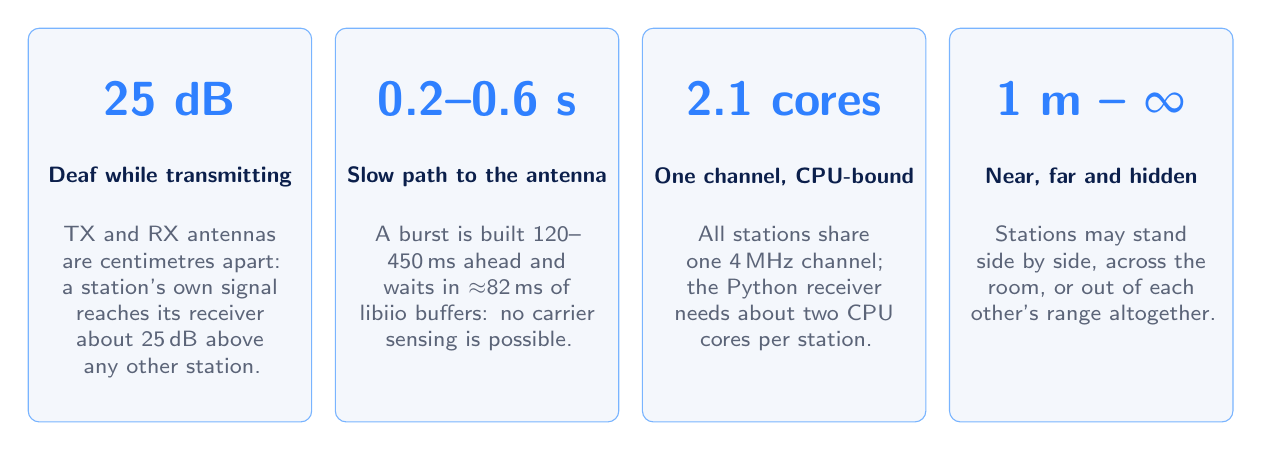
\begin{tikzpicture}[
  fact/.style={draw=wlsky,fill=wlpale,rounded corners=4pt,minimum width=36mm,minimum height=50mm,
    align=center,text width=31mm,font=\sffamily\scriptsize,inner sep=4pt}]
\foreach \i/\big/\head/\txt in {
  0/25 dB/Deaf while transmitting/{TX and RX antennas are centimetres apart: a station's own signal reaches its receiver about 25\,dB above any other station.},
  1/0.2--0.6 s/Slow path to the antenna/{A burst is built 120--450\,ms ahead and waits in $\approx$82\,ms of libiio buffers: no carrier sensing is possible.},
  2/2.1 cores/{One channel, CPU-bound}/{All stations share one 4\,MHz channel; the Python receiver needs about two CPU cores per station.},
  3/1 m -- $\infty$/{Near, far and hidden}/{Stations may stand side by side, across the room, or out of each other's range altogether.}}{
  \node[fact] (f\i) at (\i*39mm,0) {};
  \node[font=\sffamily\bfseries\LARGE,text=wlblue] at ([yshift=-9mm]f\i.north) {\big};
  \node[font=\sffamily\bfseries\footnotesize,text=wlnavy,text width=33mm,align=center] at ([yshift=-19mm]f\i.north) {\head};
  \node[font=\sffamily\footnotesize,text=wlgrey,text width=32mm,align=center,anchor=north] at ([yshift=-24mm]f\i.north) {\txt};
}
\end{tikzpicture}
\caption{The four hardware facts that shaped the design of WaveLink.}\label{fig:facts}
\end{figure}

The first fact rules out any scheme in which a station receives while it transmits on the same
frequency. The second rules out listen-before-talk (CSMA): by the time a burst reaches the air, the
channel state it was based on is hundreds of milliseconds old. The third makes receiver CPU a
first-class design resource. The fourth means that the near--far problem and hidden stations must
be handled by the protocol. \Cref{ch:background} shows how these facts lead to our
time-division CDMA (TD-CDMA) design.

\section{Contributions}
The main technical contributions of the project are:
\begin{itemize}
  \item a DS-CDMA physical layer as a 68-block GNU Radio flowgraph, with Golay-protected headers,
        three modulations, the 5G NR LDPC code at four rates and a receiver that tolerates
        $\pm\SI{16}{kHz}$ carrier offset and \SI{30}{ppm} clock offset;
  \item a link layer with two-level addressing, fragmentation, selective-repeat ARQ, adaptive
        modulation and coding, four priority classes and closed-loop transmit power control;
  \item \emph{TD-CDMA}, a medium-access scheme in which slots are kept in radio samples, the
        transmit-to-receive offset of each radio is measured from its own bursts, and code division
        inside each slot lets one transmitter serve every other station at once;
  \item one-hop relaying driven by link tables carried in every slot header;
  \item a complete application: chat, encryption, media quality selection, a radio dashboard, and
        a game center with UNO and a real-time race over the same radio link;
  \item three test environments (a numpy channel simulator, a GNU Radio channel simulation and
        emulated ANTSDRs running the unchanged flowgraph) and automated suites for every layer.
\end{itemize}

\section{Organisation of this report}
\Cref{ch:background} reviews the theory behind our choices and compares multiple-access schemes.
\Cref{ch:arch} presents the system architecture. \Cref{ch:phy,ch:mac,ch:tdcdma,ch:app} describe the
methodology layer by layer: physical layer, link layer, TD-CDMA medium access and relaying, and
the application. \Cref{ch:impl} explains how the system was implemented and verified, and
\cref{ch:results} presents the results. \Cref{ch:discussion} discusses the challenges, limitations
and future work, and \cref{ch:conclusion} concludes.

%% =====================================================================
\chapter{Background and Design Rationale}\label{ch:background}
%% =====================================================================

\section{Direct-sequence spread spectrum}\label{sec:dsss}
In direct-sequence spread spectrum (DS-SS) each data symbol $a_k$ is multiplied by a fast binary
sequence (the \emph{code}) of $N$ chips $c_m\in\{\pm1\}$ before pulse shaping:
\begin{equation}
  s(t)=\sum_{k} a_k \sum_{m=0}^{N-1} c_m\, p\!\left(t-kT_s-mT_c\right),\qquad T_s=N\,T_c ,
  \label{eq:dsss}
\end{equation}
where $T_c$ is the chip period, $T_s$ the symbol period and $p(t)$ a root-raised-cosine (RRC)
pulse. The receiver correlates the received signal with the same code. The wanted symbol adds
coherently over $N$ chips, while noise and signals spread with other codes add incoherently.
The resulting gain in signal-to-noise ratio is the \emph{processing gain}
\begin{equation}
  G_p = 10\log_{10} N \quad\Rightarrow\quad \frac{E_s}{N_0}=\frac{E_c}{N_0}+G_p .
  \label{eq:pg}
\end{equation}
With $N=31$ chips, $G_p=\SI{14.9}{dB}$: a burst whose SNR per chip is \SI{-11}{dB} still yields a
despread symbol SNR of about \SI{4}{dB}, enough to detect it. In WaveLink the chip rate is
$R_c=1/T_c=\SI{2}{Mchip/s}$, so the symbol rate is $R_s=R_c/31=\SI{64.5}{ksymbol/s}$ and the occupied
bandwidth is $R_c(1+\alpha)=\SI{2.7}{MHz}$ for a roll-off $\alpha=0.35$, inside the \SI{4}{MHz}
channel.

\section{Gold codes}\label{sec:gold}
Codes for code-division multiple access (CDMA) need a sharp autocorrelation peak (for timing
acquisition) and low cross-correlation with each other (for separation). Gold codes~\cite{gold1967}
are formed by adding, modulo 2, two \emph{preferred} maximal-length sequences of degree $n$ at all
$2^n-1$ relative shifts; together with the two sequences themselves this gives $2^n+1$ codes of
length $N=2^n-1$. Their periodic cross-correlation takes only three values,
\begin{equation}
  \theta_{xy}(\tau)\in\{-1,\ -t(n),\ t(n)-2\},\qquad t(n)=2^{\lfloor (n+2)/2\rfloor}+1 .
\end{equation}
For $n=5$ we get $N=31$, 33 codes and $t(5)=9$, so every cross-correlation is at most $9/31$, or
\SI{-10.7}{dB} below the peak. \Cref{fig:gold} shows the auto- and cross-correlation of two codes
from the set our code generator (\code{codes.py}) produces. Code~0 is reserved for broadcasts; a
station with address $N$ receives on code $N$.

\begin{figure}[htbp]
\centering
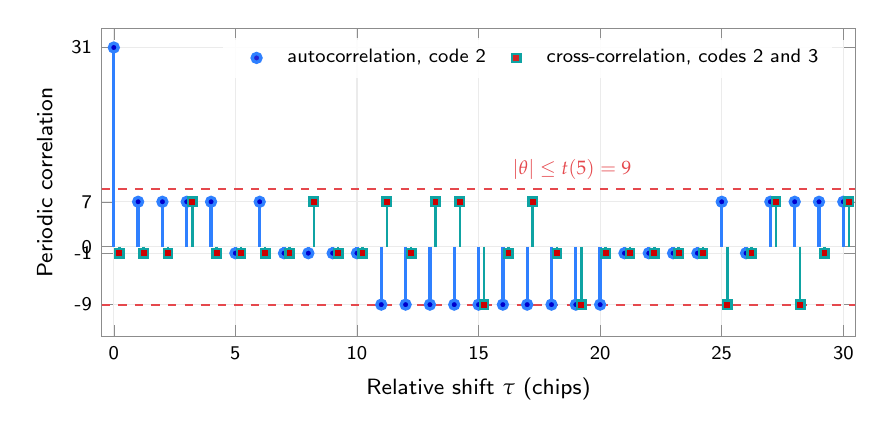
\begin{tikzpicture}
\begin{axis}[wl,width=0.92\linewidth,height=55mm,xmin=-0.5,xmax=30.5,ymin=-14,ymax=34,
  xlabel={Relative shift $\tau$ (chips)},ylabel={Periodic correlation},ytick={-9,-1,7,31},
  legend pos=north east,legend columns=2,extra y ticks={0},extra y tick style={grid style={draw=black!30}}]
\addplot+[ycomb,wlblue,mark=*,mark size=1.6pt,line width=1.2pt] coordinates {
(0,31)(1,7)(2,7)(3,7)(4,7)(5,-1)(6,7)(7,-1)(8,-1)(9,-1)(10,-1)(11,-9)(12,-9)(13,-9)(14,-9)(15,-9)(16,-9)(17,-9)(18,-9)(19,-9)(20,-9)(21,-1)(22,-1)(23,-1)(24,-1)(25,7)(26,-1)(27,7)(28,7)(29,7)(30,7)};
\addlegendentry{autocorrelation, code 2}
\addplot+[ycomb,wlteal,mark=square*,mark size=1.5pt,line width=0.9pt,xshift=2pt] coordinates {
(0,-1)(1,-1)(2,-1)(3,7)(4,-1)(5,-1)(6,-1)(7,-1)(8,7)(9,-1)(10,-1)(11,7)(12,-1)(13,7)(14,7)(15,-9)
(16,-1)(17,7)(18,-1)(19,-9)(20,-1)(21,-1)(22,-1)(23,-1)(24,-1)(25,-9)(26,-1)(27,7)(28,-9)(29,-1)(30,7)};
\addlegendentry{cross-correlation, codes 2 and 3}
\addplot[wlcoral,dashed,line width=0.7pt,forget plot] coordinates {(-0.5,9)(30.5,9)};
\addplot[wlcoral,dashed,line width=0.7pt,forget plot] coordinates {(-0.5,-9)(30.5,-9)};
\node[font=\sffamily\scriptsize,text=wlcoral,anchor=south west] at (axis cs:16,9) {$|\theta|\le t(5)=9$};
\end{axis}
\end{tikzpicture}
\caption{Periodic auto- and cross-correlation of 31-chip Gold codes from the WaveLink code set.
Side lobes and cross-correlation never exceed $9/31$ ($-10.7$\,dB).}\label{fig:gold}
\end{figure}

\section{Multiple access for a small SDR network}\label{sec:ma}
Four stations sharing one channel can be separated in frequency (FDMA), in time (TDMA), by code
(CDMA), by contention (ALOHA, CSMA/CA) or by a combination. \Cref{tab:ma} evaluates the candidates
against the four facts of \cref{sec:facts} and two needs of the application: reaching several
destinations at once, and the peak rate one link can obtain.

\begin{table}[htbp]
\centering\small
\caption{Multiple-access schemes against the hardware facts (\yes\ works, \partly\ partly, \no\ fails).}\label{tab:ma}
\setlength{\tabcolsep}{3.5pt}
\begin{tabularx}{\linewidth}{@{}>{\bfseries\raggedright\arraybackslash}p{27mm}CCCCCC@{}}
\toprule
Scheme & Deaf while sending & 0.2--0.6\,s TX latency & Near--far & Hidden stations & Many destinations at once & Peak rate per link\\
\midrule
CSMA/CA~\cite{ieee80211} & \partly\ no collision detection & \no\ stale sensing & \yes & \no\ collisions & \no & \yes\ full\\
FDMA & \partly\ front-end range & \yes & \partly\ leakage & \no & \no\ one channel each & \no\ $\tfrac14$ band\\
TDMA, one code & \yes & \yes\ sample timing & \yes & \partly\ needs relays & \no\ one at a time & \yes\ full\\
Spread ALOHA~\cite{abramson1970} & \no\ 755--900 resends & \yes & \partly\ power control & \no\ unreachable & \yes & \yes\ full\\
OFDMA & \partly\ scheduling & \no\ central scheduler & \partly\ power control & \no & \yes & \partly\ share\\
\rowcolor{wllight}TD-CDMA (ours) & \yes\ one on air & \yes\ slots in samples & \yes\ one transmitter & \yes\ one-hop relay & \yes\ code per destination & \partly\ $\approx$80\,\% of ALOHA\\
\bottomrule
\end{tabularx}
\end{table}

CSMA fails because sensing is 0.2--\SI{0.6}{s} stale and a spread signal sits below the noise
floor, so there is little to sense. FDMA gives each link a quarter of the band and still needs a
receiver per channel. A plain TDMA network works, but serves one destination per slot. Spread
ALOHA (every station transmits whenever it wishes, separated only by codes) was our first design;
it collapses on real radios because a station loses everything that arrives while it is
transmitting. OFDMA would need a central scheduler with closed-loop timing and frequency control,
which the transmit latency makes impractical.

\emph{TD-CDMA} keeps the rule of TDMA (one transmitter on the air at a time) and adds CDMA inside
each slot: a station sends to every destination at once, each on the destination's own code, and
every receiver despreads only its own code and the broadcast code. Nobody transmits while another
station is sending, so self-deafness and the near--far problem disappear; codes still provide
physical-layer addressing, multi-destination transmission and \SI{14.9}{dB} of processing gain.
The cost is that a single link obtains about 80\,\% of the speed it would get under spread ALOHA,
because each cycle also contains the other stations' slots, a join slot and slot headers.

\section{Channel coding and link adaptation}\label{sec:coding-bg}
Low-density parity-check (LDPC) codes~\cite{gallager1962} approach channel capacity with iterative
message-passing decoding. The 5G New Radio data channel uses quasi-cyclic LDPC codes defined by two
base graphs~\cite{ts38212,richardson2018}; base graph~1 (BG1) is a $46\times68$ protograph that is
\emph{lifted} by a factor $Z\in\{2,\ldots,384\}$ into a sparse parity-check matrix. Its
rate-compatible structure lets one mother code serve every rate from about $\tfrac13$ to
$\tfrac89$ by puncturing. We use BG1 at rates $\tfrac12$, $\tfrac23$, $\tfrac34$ and $\tfrac56$, decoded with
the layered~\cite{hocevar2004} normalised min-sum algorithm~\cite{chen2002}.

The PHY header is protected by the extended Golay $(24,12)$ code~\cite{golay1949,macwilliams1977},
whose minimum distance of 8 and small codebook (\num{4096} words) allow exact soft
maximum-likelihood decoding.

The capacity of an AWGN channel with symbol SNR $\gamma=E_s/N_0$ is $C=\log_2(1+\gamma)$ bits per
symbol~\cite{shannon1948}. No single modulation and code rate is efficient over the whole range of
SNRs a lab link experiences (from a few dB across the room to over \SI{40}{dB} for stations side by
side), so the sender chooses the rate per frame from the SNR the receiver reports: \emph{adaptive
modulation and coding} (AMC). Combined with CRC-32 error detection and ARQ, this is a type-I hybrid
ARQ scheme: the code corrects most errors, the CRC detects the rest and ARQ repairs them.

%% =====================================================================
\chapter{System Architecture}\label{ch:arch}
%% =====================================================================

\section{Network overview}
A WaveLink network consists of two to four \emph{stations}. Each station is one PC running the
WaveLink software and one ANTSDR\,E200 connected by Gigabit Ethernet (\cref{fig:network}). The
ANTSDR\,E200 combines an Analog Devices AD9361 (or AD9363) $2\times2$ transceiver with a Xilinx
Zynq-7020, runs Pluto-compatible libiio firmware and is driven from GNU Radio through the gr-iio
PlutoSDR blocks~\cite{antsdr,ad9361,libiio}. The user interacts with the station through a web
browser served by the station itself, so no internet connection is needed.

\begin{figure}[htbp]
\centering
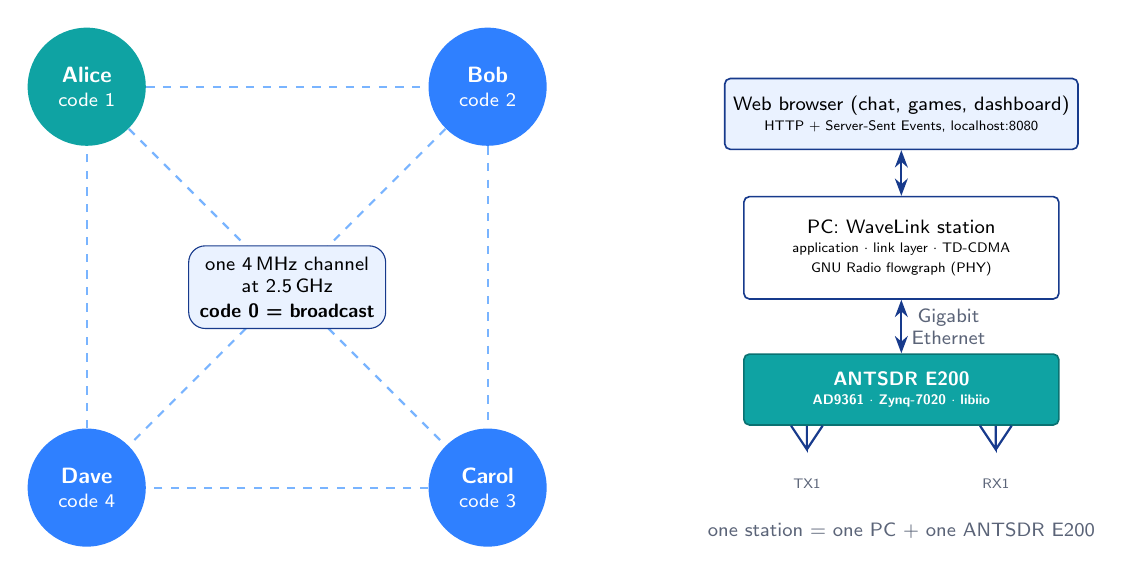
\begin{tikzpicture}[node distance=10mm]
  \def\R{36mm}
  \foreach \name/\code/\ang/\col in {Alice/1/135/wlteal,Bob/2/45/wlblue,Carol/3/-45/wlblue,Dave/4/-135/wlblue}{
    \node[station,fill=\col,minimum size=15mm,font=\sffamily\footnotesize\bfseries] (\name) at (\ang:\R) {\name\\[-1pt]{\scriptsize\mdseries code \code}};
  }
  \foreach \a/\b in {Alice/Bob,Bob/Carol,Carol/Dave,Dave/Alice,Alice/Carol,Bob/Dave}
    \draw[wlsky,dashed,line width=0.8pt] (\a) -- (\b);
  \node[draw=wldeep,fill=wllight,rounded corners=6pt,font=\sffamily\scriptsize,align=center,inner sep=4pt]
    at (0,0) {one 4\,MHz channel\\at 2.5\,GHz\\[1pt]\textbf{code 0 = broadcast}};
  % station detail
  \begin{scope}[shift={(78mm,0)}]
    \node[blk,minimum width=40mm,minimum height=9mm] (br) at (0,22mm) {Web browser (chat, games, dashboard)\\[-1pt]{\tiny HTTP + Server-Sent Events, localhost:8080}};
    \node[blk,minimum width=40mm,minimum height=13mm,fill=white] (pc) at (0,5mm) {PC: WaveLink station\\[-1pt]{\tiny application $\cdot$ link layer $\cdot$ TD-CDMA}\\[-1pt]{\tiny GNU Radio flowgraph (PHY)}};
    \node[radio,minimum width=40mm,minimum height=9mm] (sdr) at (0,-13mm) {ANTSDR E200\\[-1pt]{\tiny AD9361 $\cdot$ Zynq-7020 $\cdot$ libiio}};
    \draw[flow,<->] (br) -- (pc);
    \draw[flow,<->] (pc) -- node[right,note]{Gigabit\\Ethernet} (sdr);
    \node[font=\sffamily\tiny,text=wlgrey] (tx) at (-12mm,-25mm) {TX1};
    \node[font=\sffamily\tiny,text=wlgrey] (rx) at (12mm,-25mm) {RX1};
    \draw[wldeep,line width=0.8pt] ([xshift=-12mm]sdr.south) -- ++(0,-3mm) -- ++(-2mm,3mm) ++(2mm,-3mm) -- ++(2mm,3mm);
    \draw[wldeep,line width=0.8pt] ([xshift=12mm]sdr.south) -- ++(0,-3mm) -- ++(-2mm,3mm) ++(2mm,-3mm) -- ++(2mm,3mm);
    \node[note] at (0,-31mm) {one station = one PC + one ANTSDR E200};
  \end{scope}
\end{tikzpicture}
\caption{A WaveLink network of four stations (left) and the contents of one station (right). Every
pair of stations can communicate; station $N$ despreads only Gold code $N$ and the broadcast code~0.}
\label{fig:network}
\end{figure}

\section{Layered architecture}\label{sec:layers}
The software follows a strict layering (\cref{fig:layers}). Each layer communicates only with its
neighbours through narrow interfaces, which allowed the four members of the team to work in
parallel and allowed each layer to be tested against simulated neighbours.

\begin{figure}[htbp]
\centering
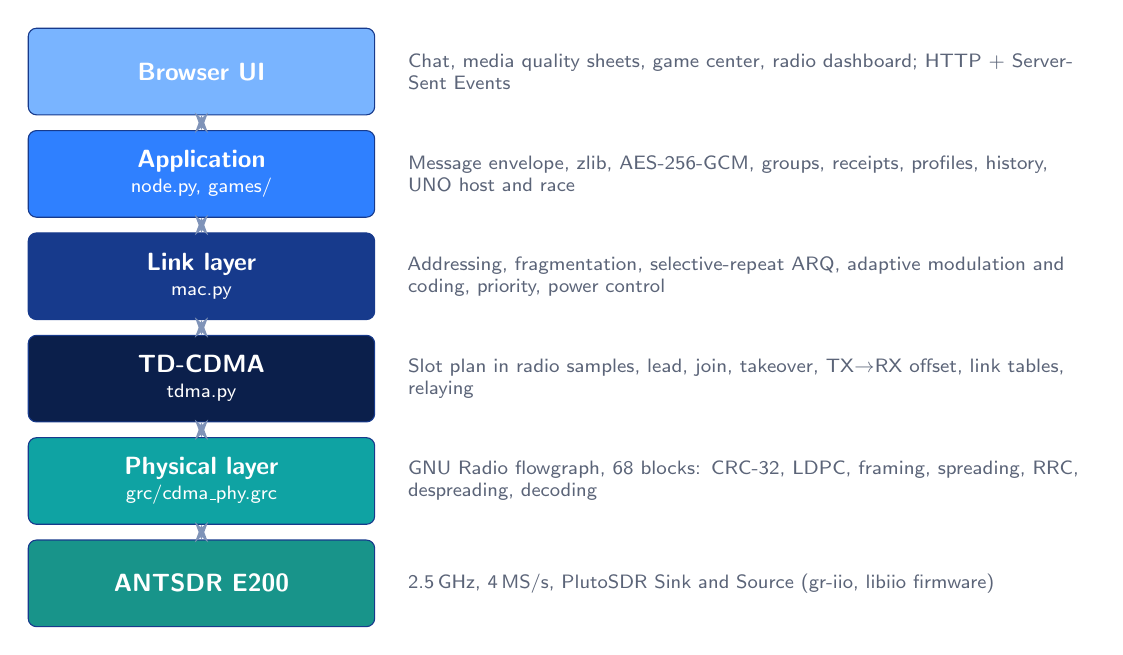
\begin{tikzpicture}[
  layer/.style={draw=wldeep,rounded corners=3pt,minimum width=44mm,minimum height=11mm,font=\sffamily\small\bfseries,
     text=white,align=center},
  desc/.style={font=\sffamily\scriptsize,text=wlgrey,anchor=west,text width=86mm,align=left}]
  \foreach \y/\t/\f/\d/\c in {
    0/Browser UI/static/{Chat, media quality sheets, game center, radio dashboard; HTTP + Server-Sent Events}/wlsky,
    -13/Application\\[-2pt]{\scriptsize\mdseries node.py, games/}/node/{Message envelope, zlib, AES-256-GCM, groups, receipts, profiles, history, UNO host and race}/wlblue,
    -26/Link layer\\[-2pt]{\scriptsize\mdseries mac.py}/mac/{Addressing, fragmentation, selective-repeat ARQ, adaptive modulation and coding, priority, power control}/wldeep,
    -39/TD-CDMA\\[-2pt]{\scriptsize\mdseries tdma.py}/tdma/{Slot plan in radio samples, lead, join, takeover, TX$\to$RX offset, link tables, relaying}/wlnavy,
    -52/Physical layer\\[-2pt]{\scriptsize\mdseries grc/cdma\_phy.grc}/phy/{GNU Radio flowgraph, 68 blocks: CRC-32, LDPC, framing, spreading, RRC, despreading, decoding}/wlteal,
    -65/ANTSDR E200/sdr/{2.5\,GHz, 4\,MS/s, PlutoSDR Sink and Source (gr-iio, libiio firmware)}/wlmint!70!black}{
    \node[layer,fill=\c] (\f) at (0,\y mm) {\t};
    \node[desc] at (25mm,\y mm) {\d};
  }
  \foreach \a/\b in {static/node,node/mac,mac/tdma,tdma/phy,phy/sdr}
    \draw[<->,wlsteel,line width=0.8pt] (\a) -- (\b);
\end{tikzpicture}
\caption{Layered software architecture of a WaveLink station.}\label{fig:layers}
\end{figure}

\Cref{tab:modules} maps the layers to the source modules. The station software is about
\num{10600} lines of Python, the browser front end about \num{6600} lines of JavaScript, CSS and
HTML, and the test suites about \num{5300} lines.

\begin{table}[htbp]
\centering\small
\caption{Main software modules.}\label{tab:modules}
\begin{tabularx}{\linewidth}{@{}>{\ttfamily\small}p{35mm}L>{\raggedleft\arraybackslash}p{14mm}@{}}
\toprule
\textrm{\textbf{Module}} & \textbf{Responsibility} & \textbf{Lines}\\
\midrule
grc/cdma\_phy.grc & The station PHY: GNU Radio flowgraph compiled with \code{grcc} at start-up & --\\
grc\_phy.py & Compiles and loads the flowgraph; cores of the Embedded Python blocks & 674\\
modem.py & Burst modulator and streaming multi-code demodulator & 866\\
ldpc.py, nr\_bg1.py & 5G NR LDPC encoder, rate matching, interleaver, layered min-sum decoder & 596\\
codes.py, golay.py & Gold codes, preambles, RRC taps; Golay (24,12) soft decoding & 179\\
mac.py & Link layer: ARQ, AMC table, power control, spread ALOHA & \num{1259}\\
tdma.py & TD-CDMA: slot plan, lead, join, takeover, TX$\to$RX offset, relaying & \num{1611}\\
node.py, crypto.py & Application: envelope, encryption, groups, receipts, profiles & \num{1054}\\
games/ & Game center: rooms, clock sync, UNO rules engine and host, race & \num{1808}\\
radio\_sim.py, fake\_antsdr.py & Channel simulator; emulated ANTSDR blocks and air & \num{1336}\\
web/ & Station web server and browser UI & \num{6600}\\
\bottomrule
\end{tabularx}
\end{table}

\section{Air-interface parameters}
\Cref{tab:phy} summarises the air interface. All rates follow from the sample rate, the samples per
chip and the code length, which are variables of the flowgraph.

\begin{table}[htbp]
\centering\small
\caption{WaveLink air-interface parameters.}\label{tab:phy}
\begin{tabularx}{0.88\linewidth}{@{}lL@{}}
\toprule
\textbf{Parameter} & \textbf{Value}\\
\midrule
Carrier frequency & \SI{2.500}{GHz}\\
Sample rate / RF bandwidth & \SI{4}{MS/s} / \SI{4}{MHz}\\
Chip rate, samples per chip & \SI{2}{Mchip/s}, 2\\
Spreading & 31-chip Gold codes, 33 codes, processing gain \SI{14.9}{dB}\\
Symbol rate & \SI{64.5}{ksymbol/s} ($T_s=\SI{15.5}{\micro s}$)\\
Pulse shape & Root-raised cosine, $\alpha=0.35$, span 8 chips; occupied bandwidth \SI{2.7}{MHz}\\
Preamble & 48 known BPSK symbols, different for every code\\
Header & 24 bits (length 11, modulation 2, code rate 3, CRC-8), two Golay (24,12) words, 48 BPSK symbols\\
Payload modulation & BPSK, QPSK or 16-QAM (Gray mapped), chosen per frame\\
Channel code & 5G NR LDPC BG1, rates $\tfrac12,\tfrac23,\tfrac34,\tfrac56$ or uncoded; one codeword per frame\\
Maximum frame & \num{1024} bytes (link-layer frame + CRC-32)\\
Payload bit rate & \SI{64.5}{kb/s} (QPSK $\tfrac12$) to \SI{258}{kb/s} (uncoded 16-QAM)\\
\bottomrule
\end{tabularx}
\end{table}

\section{A message's path through the system}\label{sec:journey}
\Cref{fig:hibob} follows the text ``Hi Bob!'' from Alice to Bob, with the actual sizes produced by our
code. The 7-byte text becomes a 73-byte application envelope (kind, identifier, timestamp and other
metadata), an 87-byte link-layer frame (10 header bytes and a CRC-32), a 928-bit LDPC codeword at
16-QAM rate $\tfrac34$, and a burst of 336 symbols (48 preamble, 48 header, 232 payload and 8 padding
symbols) that occupies the air for \SI{5.2}{ms}.

\begin{figure}[htbp]
\centering
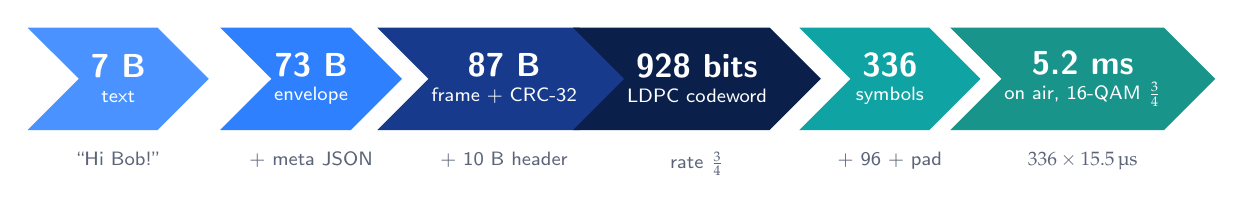
\begin{tikzpicture}[
  chev/.style={shape=signal,signal to=east,signal from=west,draw=none,minimum height=13mm,
    minimum width=23mm,font=\sffamily\scriptsize,text=white,align=center,inner sep=1pt}]
  \foreach \i/\a/\b/\c in {0/7 B/text/wlblue!65!wlsky,1/73 B/envelope/wlblue,2/87 B/frame + CRC-32/wldeep,
     3/928 bits/LDPC codeword/wlnavy,4/336/symbols/wlteal,5/5.2 ms/{on air, 16-QAM $\tfrac34$}/wlmint!70!black}
    \node[chev,fill=\c] at (\i*24.5mm,0) {\textbf{\large\a}\\[1pt]\b};
  \foreach \i/\t in {0/{``Hi Bob!''},1/{+ meta JSON},2/{+ 10 B header},3/{rate $\tfrac34$},4/{+ 96 + pad},5/{$336\times\SI{15.5}{\micro s}$}}
    \node[note,anchor=north] at (\i*24.5mm,-8mm) {\t};
\end{tikzpicture}
\caption{Encapsulation of the message ``Hi Bob!'' from Alice to Bob, layer by layer.}\label{fig:hibob}
\end{figure}

A photo follows the same path with more steps: the browser re-encodes it at the chosen quality, the
application seals the envelope with AES-256-GCM, the link layer cuts \num{1009}-byte fragments and
chooses the fastest rate Bob's last SNR report allows, and in Alice's next slot the fragments go
out on Bob's code while her slot header goes out on the broadcast code. Bob reassembles the
fragments, acknowledges them in his next two slot headers (so Alice resends only gaps), decrypts the
envelope and pushes the photo to his browser. The following four chapters describe each step.
%% =====================================================================
\chapter{Physical Layer Design}\label{ch:phy}
%% =====================================================================

\section{The GNU Radio flowgraph}\label{sec:grc}
The physical layer of every station is a single GNU Radio Companion flowgraph,
\code{grc/cdma\_phy.grc}~\cite{gnuradio}. When a station starts, the application compiles the file
with \code{grcc}, imports the generated top block, sets its parameters (node identifier, ANTSDR
address, carrier, gains, transmit buffer) and runs it. The link layer talks to the flowgraph only
through two message ports: \emph{MAC$\to$PHY} and \emph{PHY$\to$MAC}. Everything in between is the
flowgraph, so the radio processing can be inspected, modified and re-run in the GRC editor without
touching the rest of the system.

The flowgraph contains 68 processing blocks. Sixty-one are stock GNU Radio blocks (Stream CRC32,
Chunks to Symbols, Repeat, Vector Source, Multiply, PDU and tagged-stream converters, PDU Filter,
Constellation Soft Decoder, Interpolating FIR, FFT Filter and the gr-iio PlutoSDR Sink and Source).
Seven are Embedded Python blocks that hold our own signal processing (\cref{tab:epy}). There are five
transmit \emph{code lanes} (codes 0--4) and three receive branches (BPSK, QPSK, 16-QAM).
\Cref{fig:grc} shows the signal path; \cref{fig:grcrender} in \cref{app:grc} shows the saved layout of the
file itself.

\begin{figure}[htbp]
\centering
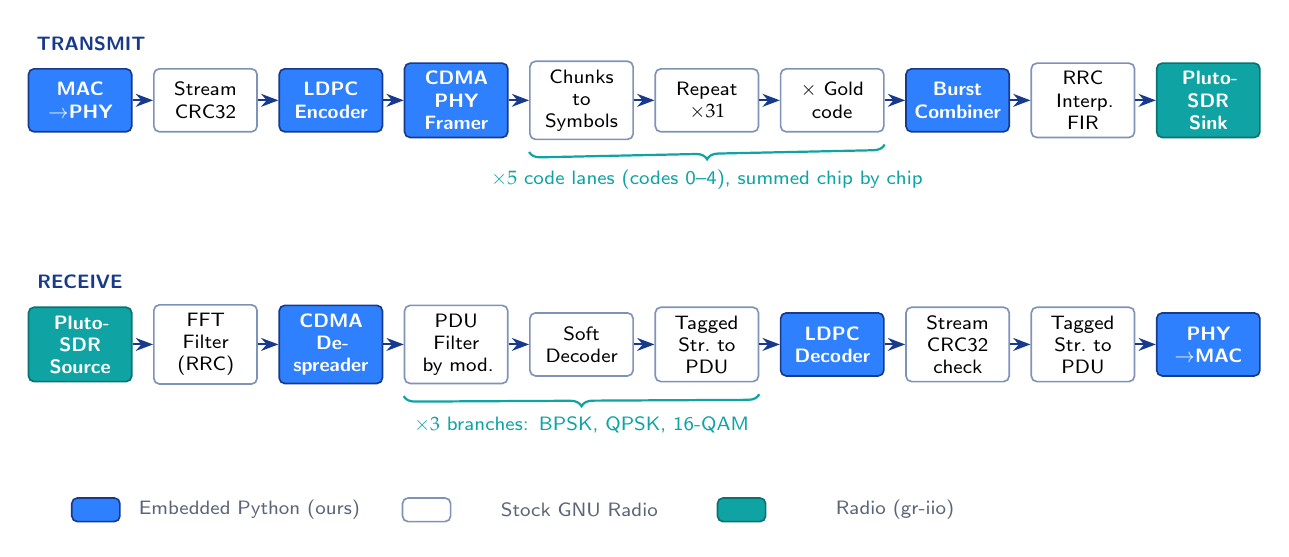
\begin{tikzpicture}[node distance=2.2mm and 2.6mm,
  every node/.append style={minimum width=12mm,minimum height=11mm,text width=11mm}]
  \node[epy] (t1) {MAC\\$\to$PHY};
  \node[lbl,minimum width=0,minimum height=0,text width=20mm,anchor=south west] at ([yshift=1mm]t1.north west) {TRANSMIT};
  \node[stock,right=of t1] (t2) {Stream CRC32};
  \node[epy,right=of t2] (t3) {LDPC Encoder};
  \node[epy,right=of t3] (t4) {CDMA PHY Framer};
  \node[stock,right=of t4] (t5) {Chunks to Symbols};
  \node[stock,right=of t5] (t6) {Repeat $\times31$};
  \node[stock,right=of t6] (t7) {$\times$ Gold code};
  \node[epy,right=of t7] (t8) {Burst Combiner};
  \node[stock,right=of t8] (t9) {RRC Interp.\ FIR};
  \node[radio,right=of t9] (t10) {Pluto\-SDR Sink};
  \foreach \a/\b in {t1/t2,t2/t3,t3/t4,t4/t5,t5/t6,t6/t7,t7/t8,t8/t9,t9/t10} \draw[flow] (\a) -- (\b);
  \draw[decorate,decoration={brace,mirror,amplitude=4pt},wlteal,line width=0.8pt]
    ([yshift=-1.5mm]t5.south west) -- node[below=4pt,note,text=wlteal,text width=60mm,minimum height=0]{$\times5$ code lanes (codes 0--4), summed chip by chip} ([yshift=-1.5mm]t7.south east);
  \begin{scope}[yshift=-31mm]
  \node[radio] (r1) {Pluto\-SDR Source};
  \node[lbl,minimum width=0,minimum height=0,text width=20mm,anchor=south west] at ([yshift=1mm]r1.north west) {RECEIVE};
  \node[stock,right=of r1] (r2) {FFT Filter (RRC)};
  \node[epy,right=of r2] (r3) {CDMA De\-spreader};
  \node[stock,right=of r3] (r4) {PDU Filter by mod.};
  \node[stock,right=of r4] (r5) {Soft Decoder};
  \node[stock,right=of r5] (r6) {Tagged Str.\ to PDU};
  \node[epy,right=of r6] (r7) {LDPC Decoder};
  \node[stock,right=of r7] (r8) {Stream CRC32 check};
  \node[stock,right=of r8] (r9) {Tagged Str.\ to PDU};
  \node[epy,right=of r9] (r10) {PHY\\$\to$MAC};
  \foreach \a/\b in {r1/r2,r2/r3,r3/r4,r4/r5,r5/r6,r6/r7,r7/r8,r8/r9,r9/r10} \draw[flow] (\a) -- (\b);
  \draw[decorate,decoration={brace,mirror,amplitude=4pt},wlteal,line width=0.8pt]
    ([yshift=-1.5mm]r4.south west) -- node[below=4pt,note,text=wlteal,text width=60mm,minimum height=0]{$\times3$ branches: BPSK, QPSK, 16-QAM} ([yshift=-1.5mm]r6.south east);
  \end{scope}
  \node[epy,minimum width=4mm,text width=4mm,minimum height=3mm] (k1) at (0.2,-52mm) {};
  \node[note,anchor=west,text width=30mm,minimum width=0,minimum height=0] at (k1.east) {Embedded Python (ours)};
  \node[stock,minimum width=4mm,text width=4mm,minimum height=3mm] (k2) at (4.4,-52mm) {};
  \node[note,anchor=west,text width=30mm,minimum width=0,minimum height=0] at (k2.east) {Stock GNU Radio};
  \node[radio,minimum width=4mm,text width=4mm,minimum height=3mm] (k3) at (8.4,-52mm) {};
  \node[note,anchor=west,text width=30mm,minimum width=0,minimum height=0] at (k3.east) {Radio (gr-iio)};
\end{tikzpicture}
\caption{Signal path of the PHY flowgraph \code{cdma\_phy.grc}. Code lanes and receive branches are drawn once.}
\label{fig:grc}
\end{figure}

\begin{table}[htbp]
\centering\small
\caption{The seven Embedded Python blocks of the flowgraph.}\label{tab:epy}
\begin{tabularx}{\linewidth}{@{}>{\bfseries\raggedright\arraybackslash}p{30mm}L@{}}
\toprule
Block & Function\\
\midrule
MAC$\to$PHY, PHY$\to$MAC & Hand frames between the link layer and the flowgraph as PDUs. Metadata: destination code, modulation and coding (e.g.\ \code{16qam-3/4}), power backoff and the exact chip at which the burst must start; on receive also SNR, CFO, LDPC iterations and the receive sample index.\\
LDPC Encoder & 5G NR LDPC encoding of frame + CRC-32, rate matching to the requested rate, 5G bit interleaver.\\
CDMA PHY Framer & Builds the burst as indices into a combined symbol table: preamble, Golay-coded header and payload symbols (BPSK 0--1, QPSK 2--5, 16-QAM 6--21).\\
CDMA Burst Combiner & Adds the five code lanes chip by chip and fills the gaps between bursts with zeros so the radio never runs dry. A burst tagged with a start chip begins exactly there; a burst that arrives late is dropped and counted.\\
CDMA Despreader & Detection, carrier-offset estimation, fractional-delay despreading with DLL, Golay header decoding and carrier tracking; outputs corrected payload symbols tagged with modulation, rate and length.\\
LDPC Decoder & De-interleaving, de-rate-matching and layered normalised min-sum decoding with early stopping.\\
\bottomrule
\end{tabularx}
\end{table}

\section{Transmitter}\label{sec:tx}

\subsection{Burst structure}
Every frame travels in its own burst (\cref{fig:burst}). A 48-symbol BPSK \emph{preamble}, different
for every code, is used for detection, timing and carrier estimation. The \emph{header} carries 24
bits (frame length 11 bits, modulation 2 bits, code rate 3 bits and a CRC-8) encoded as two extended
Golay (24,12) codewords and sent as 48 coherent BPSK symbols, so it can be decoded at low SNR before
anything is known about the payload. Because modulation and code rate are in the header, they may
change from one burst to the next. The \emph{payload} is the LDPC codeword (or the plain bits of an
uncoded frame), Gray-mapped onto BPSK, QPSK or 16-QAM and padded to a multiple of 16 symbols.

\begin{figure}[htbp]
\centering
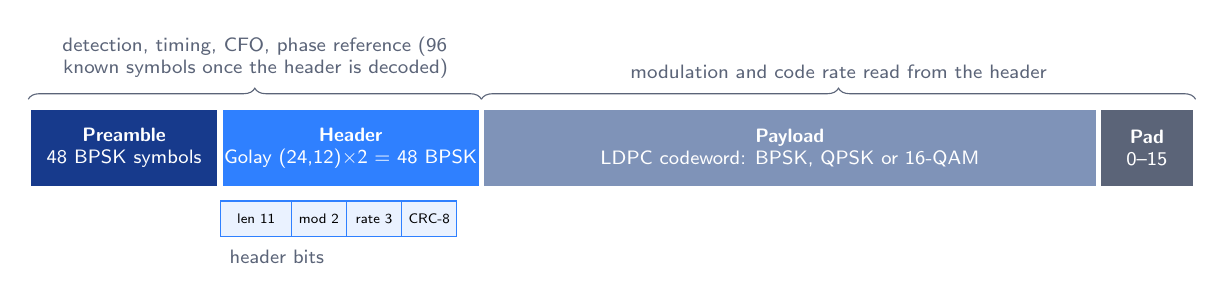
\begin{tikzpicture}[seg/.style={draw=white,line width=1pt,minimum height=10mm,font=\sffamily\scriptsize,text=white,align=center,inner sep=1pt}]
  \node[seg,fill=wldeep,minimum width=24mm,anchor=west] (p) at (0,0) {\textbf{Preamble}\\48 BPSK symbols};
  \node[seg,fill=wlblue,minimum width=30mm,anchor=west] (h) at (p.east) {\textbf{Header}\\Golay (24,12)$\times2$ = 48 BPSK};
  \node[seg,fill=wlsteel,minimum width=78mm,anchor=west] (d) at (h.east) {\textbf{Payload}\\LDPC codeword: BPSK, QPSK or 16-QAM};
  \node[seg,fill=wlgrey,minimum width=12mm,anchor=west] (x) at (d.east) {\textbf{Pad}\\0--15};
  \foreach \t/\w/\o in {len 11/9/0,mod 2/7/9,rate 3/7/16,CRC-8/7/23}
    \node[draw=wlblue,fill=wllight,font=\sffamily\tiny,minimum height=4.5mm,minimum width=\w mm,text width=\w mm-1mm,align=center,inner sep=0pt,anchor=north west]
      at ([xshift=\o mm,yshift=-1.5mm]h.south west) {\t};
  \node[note,anchor=north west] at ([yshift=-6.5mm]h.south west) {header bits};
  \draw[decorate,decoration={brace,amplitude=4pt},wlgrey] ([yshift=1mm]p.north west) -- node[above=4pt,note,text width=54mm]{detection, timing, CFO, phase reference (96 known symbols once the header is decoded)} ([yshift=1mm]h.north east);
  \draw[decorate,decoration={brace,amplitude=4pt},wlgrey] ([yshift=1mm]d.north west) -- node[above=4pt,note,text width=60mm]{modulation and code rate read from the header} ([yshift=1mm]x.north east);
\end{tikzpicture}
\caption{Structure of a WaveLink burst. Each symbol is spread by the 31 chips of the destination's Gold code.}
\label{fig:burst}
\end{figure}

\subsection{Modulation, spreading and pulse shaping}
The Framer outputs indices into a 22-entry symbol table (two BPSK, four QPSK and sixteen 16-QAM
points, all Gray mapped with unit average energy). The stock \emph{Chunks to Symbols} block maps
them to complex symbols, \emph{Repeat} holds each symbol for 31 chips, and \emph{Multiply} with a
looping \emph{Vector Source} applies the Gold code of the lane. A PDU Filter in front of each lane
selects the bursts addressed to that code. The \emph{Burst Combiner} sums the five lanes chip by
chip, so a station can transmit to several destinations simultaneously, and starts every burst on
the exact chip requested by the time-slot scheduler (\cref{ch:tdcdma}). Each burst is scaled by its
power backoff (\cref{sec:power}). Finally an interpolating FIR filter applies the RRC pulse at two
samples per chip and the PlutoSDR Sink hands the \SI{4}{MS/s} stream to the ANTSDR.

All codes in a slot are transmitted at one common level. With more than two codes in a slot the level
is reduced by $10\log_{10}(n_\text{codes}/2)$\,dB so that the sum stays at the level of two full-power
codes (RMS 0.35 of DAC full scale), which leaves about \SI{9}{dB} of headroom for 16-QAM peaks.
\Cref{fig:psd} shows the resulting spectrum, computed from bursts produced by our modulator.

\begin{figure}[htbp]
\centering
\begin{tikzpicture}
\begin{axis}[wl,width=0.9\linewidth,height=52mm,xmin=-2,xmax=2,ymin=-65,ymax=5,
  xlabel={Frequency offset from carrier (MHz)},ylabel={PSD (dB, normalised)},
  xtick={-2,-1.35,-1,0,1,1.35,2},xticklabels={$-2$,$-1.35$,$-1$,0,1,1.35,2}]
\fill[wlblue!8] (axis cs:-1.35,-65) rectangle (axis cs:1.35,5);
\addplot[wlblue,line width=1.1pt] table[x=f,y=p] {data/psd.dat};
\draw[wlcoral,dashed,line width=0.7pt] (axis cs:-1.35,-65) -- (axis cs:-1.35,5);
\draw[wlcoral,dashed,line width=0.7pt] (axis cs:1.35,-65) -- (axis cs:1.35,5);
\node[font=\sffamily\scriptsize,text=wlcoral,fill=white,inner sep=1pt] at (axis cs:0,-55) {$R_c(1+\alpha)=2.7$\,MHz};
\end{axis}
\end{tikzpicture}
\caption{Power spectral density of a WaveLink transmission (16-QAM, 2\,Mchip/s, RRC $\alpha=0.35$),
from bursts generated by the project's modulator. The signal occupies 2.7\,MHz of the 4\,MHz channel.}
\label{fig:psd}
\end{figure}

\subsection{Spreading and despreading in practice}
\Cref{fig:despread} illustrates processing gain with the actual code set. Two users transmit BPSK
symbols on codes 1 and 2 at the same time, at a chip SNR of \SI{-3}{dB} each. The received chips
(top) look like noise. Correlating with code~1 (middle) produces peaks of about $\pm31$ at symbol
boundaries that reveal user~1's data, while correlating with an unused code (bottom) produces only
noise and cross-correlation. This is how a WaveLink station ignores traffic addressed to others.

\begin{figure}[htbp]
\centering
\begin{tikzpicture}
\begin{axis}[wl,name=a1,width=0.95\linewidth,height=30mm,xmin=0,xmax=155,ymin=-4,ymax=4,
  ylabel={chips},xticklabels={},ytick={-3,0,3},title style={font=\sffamily\scriptsize,yshift=-1.5ex},
  title={Received chips: users on codes 1 and 2 plus noise (chip SNR $-3$\,dB per user)}]
\addplot[wlsteel,line width=0.5pt,const plot] table[x=n,y=r] {data/chips.dat};
\pgfplotsinvokeforeach{31,62,93,124}{\draw[black!25,dashed] (axis cs:#1,-4) -- (axis cs:#1,4);}
\end{axis}
\begin{axis}[wl,at={(a1.south west)},anchor=north west,yshift=-9mm,name=a2,width=0.95\linewidth,height=34mm,
  xmin=0,xmax=9,ymin=-45,ymax=45,ylabel={correlation},xticklabels={},ytick={-31,0,31},
  title style={font=\sffamily\scriptsize,yshift=-1.5ex},title={Sliding correlation with code 1 (the right code)}]
\addplot[wlblue,line width=0.8pt] table[x=n,y=right] {data/despread.dat};
\addplot[only marks,mark=*,mark size=1.6pt,wlcoral] table[x=n,y=right,each nth point=31] {data/despread.dat};
\end{axis}
\begin{axis}[wl,at={(a2.south west)},anchor=north west,yshift=-9mm,width=0.95\linewidth,height=34mm,
  xmin=0,xmax=9,ymin=-45,ymax=45,ylabel={correlation},xlabel={Time (symbols, 31 chips each)},ytick={-31,0,31},
  title style={font=\sffamily\scriptsize,yshift=-1.5ex},title={Sliding correlation with code 3 (a code nobody uses)}]
\addplot[wlteal,line width=0.8pt] table[x=n,y=wrong] {data/despread.dat};
\end{axis}
\end{tikzpicture}
\caption{Processing gain with the WaveLink code set: the received chips are buried in noise, but
correlating with the right code recovers the symbols (red dots at symbol boundaries); a different
code sees only noise.}
\label{fig:despread}
\end{figure}

\section{Receiver and synchronisation}\label{sec:rx}
Two independent ANTSDRs differ in carrier frequency (their \SI{40}{MHz} references are rated
$\pm\SI{2}{ppm}$, but we designed for \SI{16}{kHz} offsets at \SI{2.5}{GHz}), in sample clock and in
the arbitrary phase and timing of every burst. The receiver of the CDMA Despreader block resolves
these in the sequence of \cref{fig:rxchain}~\cite{mengali1997}.

\begin{figure}[htbp]
\centering
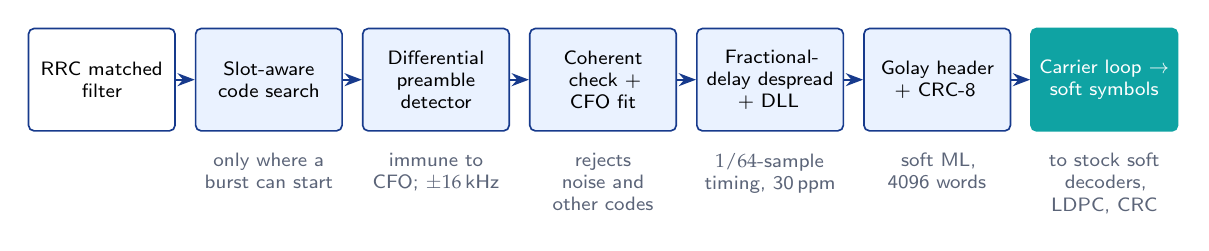
\begin{tikzpicture}[st/.style={blk,minimum width=17.5mm,text width=16.5mm,minimum height=13mm},node distance=2.4mm]
  \node[st,fill=white] (s1) {RRC matched filter};
  \node[st,right=of s1] (s2) {Slot-aware code search};
  \node[st,right=of s2] (s3) {Differential preamble detector};
  \node[st,right=of s3] (s4) {Coherent check + CFO fit};
  \node[st,right=of s4] (s5) {Fractional-delay despread + DLL};
  \node[st,right=of s5] (s6) {Golay header + CRC-8};
  \node[st,right=of s6,fill=wlteal,text=white,draw=wlteal] (s7) {Carrier loop $\to$ soft symbols};
  \foreach \a/\b in {s1/s2,s2/s3,s3/s4,s4/s5,s5/s6,s6/s7} \draw[flow] (\a) -- (\b);
  \node[note,below=1.5mm of s2,text width=17mm] {only where a burst can start};
  \node[note,below=1.5mm of s3,text width=17mm] {immune to CFO; $\pm16$\,kHz};
  \node[note,below=1.5mm of s4,text width=17mm] {rejects noise and other codes};
  \node[note,below=1.5mm of s5,text width=17mm] {$1/64$-sample timing, 30\,ppm};
  \node[note,below=1.5mm of s6,text width=17mm] {soft ML, 4096 words};
  \node[note,below=1.5mm of s7,text width=17mm] {to stock soft decoders, LDPC, CRC};
\end{tikzpicture}
\caption{Synchronisation and detection chain inside the CDMA Despreader block.}\label{fig:rxchain}
\end{figure}

\subsection{Burst detection}
For every candidate start time $\tau$ the receiver despreads the 48 preamble positions, giving
symbols $y_k(\tau)$, and computes the normalised \emph{differential} correlation
\begin{equation}
  M(\tau)=\frac{\left|\sum_{k=1}^{K-1} q_k\, y_k(\tau)\, y_{k-1}^*(\tau)\right|}{\sum_{k=0}^{K-1}|y_k(\tau)|^2},
  \qquad q_k=b_k b_{k-1},
\end{equation}
where $b_k$ are the known preamble bits and $K=48$. A carrier offset $\Delta f$ rotates each symbol
by $2\pi\Delta f T_s$ relative to the previous one; the product $y_k y_{k-1}^*$ turns this into a
constant phase, which the magnitude ignores. The detector is therefore immune to carrier offset, and
the argument of the sum gives a coarse estimate $\widehat{\Delta f}=\arg(\cdot)/(2\pi T_s)$, unambiguous
for $|\Delta f|<1/(2T_s)=\SI{32}{kHz}$. A detection requires $M\ge0.6$. Spurious detections are then
rejected in four ways: a second, coherent check of the preamble in four segments after CFO removal,
code-specific preamble patterns, a minimum frame length, and a ``ghost'' filter that rejects partial
correlation side lobes of a much stronger burst. In three seconds of pure noise on two codes the
receiver produced no detections.

\subsection{Timing, carrier and header}
After CFO removal, a phase and frequency fit over the known preamble symbols provides the phase
reference. The \emph{fractional-delay despreader} despreads each symbol at a few whole-sample offsets
and interpolates between them with an 8-tap windowed-sinc filter to $1/64$-sample
resolution~\cite{gardner1993}. This accuracy matters for 16-QAM: without it, inter-chip interference
limits the SNR to about \SI{12}{dB}. An early--late delay-locked loop tracks the sample-clock offset
between the two radios, up to \SI{30}{ppm}.

The header is decoded by soft maximum likelihood: the 24 received soft values of each Golay word
are correlated with all \num{4096} codewords and the best one is chosen. This works down to a symbol
SNR of about \SI{1}{dB}, so the header never limits a coded frame. Once the header is known, its 48
symbols become known too, and the carrier frequency is re-estimated over all 96 known symbols. A
decision-directed second-order loop anchored on these symbols then tracks the carrier through the
payload without the $90^\circ$ ambiguity of blind QPSK or 16-QAM tracking.

\subsection{Demodulation and receiver output}
The despreader outputs unit-energy payload symbols tagged with modulation, rate and length. A PDU
Filter routes them to the stock Constellation Soft Decoder for that modulation, which computes soft
bits; on the numpy PHY the equivalent is a max-log demapper,
\begin{equation}
  L(b_j)=\frac{1}{N_0}\left(\min_{s\in\mathcal{S}_j^{1}}|z-s|^2-\min_{s\in\mathcal{S}_j^{0}}|z-s|^2\right),
\end{equation}
where $\mathcal{S}_j^{b}$ is the set of points whose $j$th bit equals $b$. \Cref{fig:const} shows
despread payload symbols produced by the full receiver from bursts with a \SI{3}{kHz} carrier offset and
an arbitrary phase; panel (c) adds a second user of equal power on another code.

\begin{figure}[htbp]
\centering
\begin{subfigure}[b]{0.32\linewidth}\centering
\begin{tikzpicture}
\begin{axis}[wl,width=50mm,height=50mm,axis equal image,xmin=-1.6,xmax=1.6,ymin=-1.6,ymax=1.6,
  xtick={-1,0,1},ytick={-1,0,1},grid=both,minor tick num=0]
\addplot[only marks,mark=*,mark size=0.55pt,wlblue,opacity=0.55] table[x=i,y=q] {data/const_qpsk.dat};
\end{axis}
\end{tikzpicture}
\caption{QPSK, \EsNo\ = 12.3\,dB}
\end{subfigure}\hfill
\begin{subfigure}[b]{0.32\linewidth}\centering
\begin{tikzpicture}
\begin{axis}[wl,width=50mm,height=50mm,axis equal image,xmin=-1.4,xmax=1.4,ymin=-1.4,ymax=1.4,
  xtick={-0.95,-0.32,0.32,0.95},ytick={-0.95,-0.32,0.32,0.95},xticklabels={},yticklabels={},grid=both]
\addplot[only marks,mark=*,mark size=0.55pt,wldeep,opacity=0.55] table[x=i,y=q] {data/const_qam.dat};
\end{axis}
\end{tikzpicture}
\caption{16-QAM, \EsNo\ = 25.0\,dB}
\end{subfigure}\hfill
\begin{subfigure}[b]{0.32\linewidth}\centering
\begin{tikzpicture}
\begin{axis}[wl,width=50mm,height=50mm,axis equal image,xmin=-1.6,xmax=1.6,ymin=-1.6,ymax=1.6,
  xtick={-0.95,-0.32,0.32,0.95},ytick={-0.95,-0.32,0.32,0.95},xticklabels={},yticklabels={},grid=both]
\addplot[only marks,mark=*,mark size=0.55pt,wlteal,opacity=0.55] table[x=i,y=q] {data/const_qammui.dat};
\end{axis}
\end{tikzpicture}
\caption{16-QAM $\tfrac34$ + 2nd user: 13.6\,dB}
\end{subfigure}
\caption{Despread payload constellations from the WaveLink receiver (3\,kHz carrier offset, random
phase). In (c) an equal-power burst on another code is suppressed by about 15\,dB; the frame still
decodes at 16-QAM rate $\tfrac34$.}\label{fig:const}
\end{figure}

\section{Forward error correction}\label{sec:ldpc}

\subsection{The 5G NR LDPC code}
Every frame (link-layer frame plus CRC-32, at most \num{1024} bytes) is encoded
as \emph{one} LDPC codeword of 5G NR base graph~1~\cite{ts38212}. The $46\times68$ base matrix is
lifted by the smallest factor $Z$ from the 51 allowed sizes with $22Z\ge K$; the remaining
information positions are filled with known zeros (\emph{filler bits}) that are never transmitted.
A full \SI{1}{KB} frame uses $Z=384$; a 30-byte frame uses $Z=11$. The base-graph table
was taken from NVIDIA Sionna~\cite{sionna} and checked entry by entry against the lifted matrices of
AFF3CT~\cite{aff3ct} for all 51 lifting sizes; a unit test checks that every encoded word satisfies all
$46Z$ parity checks.

\textbf{Encoding} exploits the structure of the 5G core: the four core parity blocks follow from
the column sums of the information part, and every extension parity block is a single row sum.
\textbf{Rate matching} follows 5G redundancy version~0: the first $2Z$ systematic bits are punctured,
fillers are skipped and the first $E=\lceil K/R\rceil$ bits (rounded up to whole symbols) are sent.
Every rate is a prefix of the same mother codeword, so one matrix serves all four rates and the
decoder simply uses fewer rows at higher rates. Finally the 5G bit interleaver spreads each codeword
across the bit positions of the QPSK or 16-QAM symbols.

\subsection{Layered normalised min-sum decoding}
The decoder processes the rows of the parity-check matrix layer by layer~\cite{hocevar2004}. For check
node $c$ and variable node $v$ the message update is the normalised min-sum rule~\cite{chen2002}
\begin{equation}
  L_{c\to v}=\alpha\prod_{v'\in\mathcal{N}(c)\setminus v}\operatorname{sgn}\!\left(L_{v'\to c}\right)\cdot
  \min_{v'\in\mathcal{N}(c)\setminus v}\left|L_{v'\to c}\right|,\qquad \alpha=0.75 ,
\end{equation}
after which the posterior of each variable node is updated immediately, so later layers in the same
iteration already use it. Rows that share no variables are merged into one layer, and every layer is
processed as a single vectorised operation over its $Z$ check nodes. Decoding stops as soon as all
parity checks are satisfied, after at most 20 iterations. Because min-sum is scale-invariant, the
decoder needs no noise estimate. A \SI{1}{KB} frame decodes in 3--\SI{7}{ms} at rate $\tfrac56$ and
15--\SI{25}{ms} at rate $\tfrac12$.

\begin{algobox}{Algorithm 1: LDPC frame decoding (\code{ldpc.decode\_frame})}
\small
\begin{enumerate}[leftmargin=*,label=\arabic*.]
  \item De-interleave the $E$ soft bits; insert zeros (unknown) for the $2Z$ punctured bits and
        $+\infty$ (known zero) for the filler bits.
  \item Select the first $n_\text{rows}=n_\text{cols}-22$ rows of the lifted matrix for the rate in use.
  \item For iteration $i=1,\ldots,20$: for each layer, subtract old check messages, compute new
        messages with the normalised min-sum rule, add them to the posteriors.
  \item Stop as soon as the hard decisions satisfy every selected parity check; return the $K$
        information bits, a success flag and the iteration count.
\end{enumerate}
\end{algobox}

\subsection{Error-rate performance}
\Cref{fig:fer} shows the frame error rate of 1\,KB frames over an AWGN channel for every coded rung,
simulated with the project's own encoder, max-log demapper and decoder (up to 300 frames per point).
The waterfalls are steep, as expected for 8-kbit codewords: each code goes from almost always failing
to error-free within about \SI{0.3}{dB}. Uncoded 16-QAM is shown both simulated and from the exact
Gray-mapped bit-error probability, $P_\text{fr}=1-(1-P_b)^{8192}$; the two agree to within \SI{0.1}{dB}.

\begin{figure}[htbp]
\centering
\begin{tikzpicture}
\begin{semilogyaxis}[wl,width=0.95\linewidth,height=68mm,xmin=0,xmax=23,ymin=2e-3,ymax=1.5,
  xlabel={\EsNo\ (dB)},ylabel={Frame error rate},cycle list name=mcs,unbounded coords=jump,
  legend style={at={(0.5,1.02)},anchor=south,legend columns=4},xtick={0,2,...,22}]
\addplot table[x=esn0,y=ferplot] {data/fer_qpsk12_all.dat}; \addlegendentry{QPSK $\tfrac12$}
\addplot table[x=esn0,y=ferplot] {data/fer_qpsk34_all.dat}; \addlegendentry{QPSK $\tfrac34$}
\addplot table[x=esn0,y=ferplot] {data/fer_qpsk56_all.dat}; \addlegendentry{QPSK $\tfrac56$}
\addplot table[x=esn0,y=ferplot] {data/fer_qam12_all.dat}; \addlegendentry{16-QAM $\tfrac12$}
\addplot table[x=esn0,y=ferplot] {data/fer_qam23_all.dat}; \addlegendentry{16-QAM $\tfrac23$}
\addplot table[x=esn0,y=ferplot] {data/fer_qam34_all.dat}; \addlegendentry{16-QAM $\tfrac34$}
\addplot table[x=esn0,y=ferplot] {data/fer_qam56_all.dat}; \addlegendentry{16-QAM $\tfrac56$}
\addplot table[x=esn0,y=ferplot] {data/fer_qamunc_all.dat}; \addlegendentry{16-QAM uncoded}
\addplot[wlviolet,dashed,line width=0.8pt,mark=none,forget plot] table[x=esn0,y=fer] {data/fer_qamunc_theory.dat};
\node[font=\sffamily\scriptsize,text=wlviolet,anchor=west] at (axis cs:20.6,0.3) {theory};
\draw[<->,wlgrey,line width=0.6pt] (axis cs:11.45,0.012) -- node[below,font=\sffamily\scriptsize,text=wlgrey]{16-QAM $\tfrac56$ vs uncoded: 7.9\,dB} (axis cs:19.3,0.012);
\end{semilogyaxis}
\end{tikzpicture}
\caption{Frame error rate of 1\,KB frames on AWGN with ideal synchronisation, simulated with the
project's LDPC code. Points with no errors in 300 frames are not drawn.}\label{fig:fer}
\end{figure}

The LDPC decoder's effort falls quickly above the threshold (\cref{fig:iters}). Near the waterfall it
uses all 20 iterations; \SIrange{1}{2}{dB} above it, 3--6. The radio dashboard shows the average iteration
count per frame as a live indicator of how close a link is to its limit.

\begin{figure}[htbp]
\centering
\begin{tikzpicture}
\begin{axis}[wl,width=0.9\linewidth,height=52mm,xmin=-1,xmax=14,ymin=0,ymax=21,
  xlabel={\EsNo\ (dB)},ylabel={Mean LDPC iterations},cycle list name=mcs,
  legend style={at={(0.5,1.03)},anchor=south,legend columns=4}]
\addplot table[x=esn0,y=iters] {data/fer_qpsk12_all.dat}; \addlegendentry{QPSK $\tfrac12$}
\addplot table[x=esn0,y=iters] {data/fer_qpsk34_all.dat}; \addlegendentry{QPSK $\tfrac34$}
\addplot table[x=esn0,y=iters] {data/fer_qpsk56_all.dat}; \addlegendentry{QPSK $\tfrac56$}
\addplot table[x=esn0,y=iters] {data/fer_qam12_all.dat}; \addlegendentry{16-QAM $\tfrac12$}
\addplot table[x=esn0,y=iters] {data/fer_qam23_all.dat}; \addlegendentry{16-QAM $\tfrac23$}
\addplot table[x=esn0,y=iters] {data/fer_qam34_all.dat}; \addlegendentry{16-QAM $\tfrac34$}
\addplot table[x=esn0,y=iters] {data/fer_qam56_all.dat}; \addlegendentry{16-QAM $\tfrac56$}
\end{axis}
\end{tikzpicture}
\caption{Mean number of layered min-sum iterations per frame (maximum 20), from the same simulation.}
\label{fig:iters}
\end{figure}

\section{The modulation and coding ladder}\label{sec:ladder}
The link layer chooses among eight \emph{rungs} (\cref{tab:mcs}). Each rung's threshold is the despread
symbol SNR at which the \emph{full receiver}, including detection, synchronisation and carrier
tracking, delivers practically all 1\,KB frames, plus a margin of 0.5--\SI{1.5}{dB}. QPSK $\tfrac12$ is the
floor: it is also used for acknowledgements, beacons and broadcasts, and its low end is set by burst
detection (about \SI{4}{dB}) rather than by the code. BPSK remains available for the mid-evaluation
tools and as a forced mode.

\begin{table}[htbp]
\centering\small
\caption{The modulation and coding ladder. Rates are payload information rates on the air.}\label{tab:mcs}
\setlength{\tabcolsep}{4.5pt}
\begin{tabular}{@{}lccccc@{}}
\toprule
\textbf{Rung} & \textbf{Bits/symbol} & \textbf{Rate (kb/s)} & \textbf{AWGN, FER 10\,\%} & \textbf{Full receiver} & \textbf{Threshold}\\
\midrule
QPSK $\tfrac12$ & 1.00 & 64.5 & \SI{1.1}{dB} & \SI{5.0}{dB}$^\dagger$ & floor\\
QPSK $\tfrac34$ & 1.50 & 96.8 & \SI{4.1}{dB} & \SI{5.5}{dB} & \SI{6.0}{dB}\\
QPSK $\tfrac56$ & 1.67 & 107.5 & \SI{5.2}{dB} & \SI{6.0}{dB} & \SI{7.0}{dB}\\
16-QAM $\tfrac12$ & 2.00 & 129.0 & \SI{6.7}{dB} & \SI{9.0}{dB} & \SI{9.5}{dB}\\
16-QAM $\tfrac23$ & 2.67 & 172.0 & \SI{8.9}{dB} & \SI{10.0}{dB} & \SI{11.0}{dB}\\
16-QAM $\tfrac34$ & 3.00 & 193.5 & \SI{10.1}{dB} & \SI{11.0}{dB} & \SI{12.5}{dB}\\
16-QAM $\tfrac56$ & 3.33 & 215.1 & \SI{11.4}{dB} & \SI{12.5}{dB} & \SI{14.0}{dB}\\
16-QAM uncoded & 4.00 & 258.1 & \SI{19.3}{dB} & 20--\SI{22}{dB} & \SI{22.5}{dB}\\
\bottomrule
\multicolumn{6}{@{}l}{\footnotesize $^\dagger$ detection-limited: the code alone would decode at about 1.5\,dB.}
\end{tabular}
\end{table}

\Cref{fig:se} places the ladder against the Shannon capacity $\log_2(1+\EsNo)$. On an ideal AWGN channel
our LDPC rungs operate 1.1--\SI{1.9}{dB} from capacity at a 10\,\% frame error rate. The full
receiver, measured for practically error-free delivery rather than 10\,\% FER, needs another
0.8--\SI{2.3}{dB} for synchronisation and channel estimation (about \SI{4}{dB} for QPSK $\tfrac12$, where
burst detection sets the limit), and the thresholds add a safety margin. Uncoded 16-QAM sits \SI{7.6}{dB} from capacity,
which is the room the code exploits.

\begin{figure}[htbp]
\centering
\begin{tikzpicture}
\begin{axis}[wl,width=0.92\linewidth,height=66mm,xmin=-2,xmax=24,ymin=0,ymax=4.6,
  xlabel={\EsNo\ (dB)},ylabel={Information bits per symbol},
  legend style={at={(0.02,0.98)},anchor=north west}]
\addplot[black!70,line width=1.1pt,domain=-2:24,samples=120] {ln(1+10^(x/10))/ln(2)};
\addlegendentry{Shannon capacity $\log_2(1+E_s/N_0)$}
\addplot[only marks,mark=*,mark size=2pt,wlblue] table[x=awgn,y=bits] {data/se.dat};
\addlegendentry{our code, AWGN (FER 10\,\%)}
\addplot[only marks,mark=square*,mark size=1.9pt,wlteal] table[x=fullrx,y=bits] {data/se.dat};
\addlegendentry{full receiver}
\addplot[const plot,wlcoral,line width=1.1pt] coordinates {(5,1)(6,1.5)(7,1.6667)(9.5,2)(11,2.6667)(12.5,3)(14,3.3333)(22.5,4)(24,4)};
\addlegendentry{ladder used by the link layer}
\node[font=\sffamily\scriptsize,anchor=south,text=wlgrey] at (axis cs:20.2,4.08) {uncoded 16-QAM};
\node[font=\sffamily\scriptsize,anchor=west,text=wlgrey] at (axis cs:14.4,3.12) {16-QAM $\tfrac56$};
\node[font=\sffamily\scriptsize,anchor=west,text=wlgrey] at (axis cs:1.6,0.85) {QPSK $\tfrac12$};
\end{axis}
\end{tikzpicture}
\caption{Spectral efficiency of the WaveLink rungs against Shannon capacity: ideal decoding of our
LDPC code, the full receiver, and the thresholds the link layer uses.}\label{fig:se}
\end{figure}
%% =====================================================================
\chapter{Link Layer Design}\label{ch:mac}
%% =====================================================================
The link layer (\code{mac.py}) turns the unreliable burst service of the PHY into reliable,
prioritised delivery of messages of any size between any two stations. It is shared by both
medium-access schemes: TD-CDMA (the default, \cref{ch:tdcdma}) and the earlier spread ALOHA.

\section{Frame formats}\label{sec:frames}
All link-layer frames start with the same four bytes (type, flags, destination, source) and end
with a CRC-32 appended by the flowgraph's stock \emph{Stream CRC32} block. Six frame types exist
(\cref{tab:frames}); \cref{fig:dataframe} shows the layout of a data frame.

\begin{figure}[htbp]
\centering
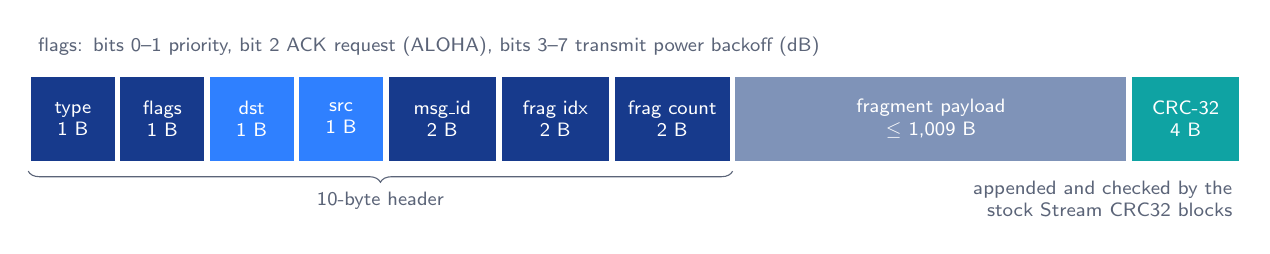
\begin{tikzpicture}[f/.style={draw=white,line width=1pt,minimum height=11mm,font=\sffamily\scriptsize,
  text=white,align=center,inner sep=1pt,anchor=west}]
  \node[f,fill=wldeep,minimum width=11mm] (a) at (0,0) {type\\1 B};
  \node[f,fill=wldeep,minimum width=11mm] (b) at (a.east) {flags\\1 B};
  \node[f,fill=wlblue,minimum width=11mm] (c) at (b.east) {dst\\1 B};
  \node[f,fill=wlblue,minimum width=11mm] (d) at (c.east) {src\\1 B};
  \node[f,fill=wldeep,minimum width=14mm] (e) at (d.east) {msg\_id\\2 B};
  \node[f,fill=wldeep,minimum width=14mm] (g) at (e.east) {frag idx\\2 B};
  \node[f,fill=wldeep,minimum width=15mm] (h) at (g.east) {frag count\\2 B};
  \node[f,fill=wlsteel,minimum width=50mm] (i) at (h.east) {fragment payload\\$\le$ 1,009 B};
  \node[f,fill=wlteal,minimum width=14mm] (j) at (i.east) {CRC-32\\4 B};
  \draw[decorate,decoration={brace,mirror,amplitude=4pt},wlgrey] ([yshift=-1mm]a.south west) -- node[below=4pt,note]{10-byte header} ([yshift=-1mm]h.south east);
  \node[note,anchor=north east,text width=34mm,align=right] at ([yshift=-1mm]j.south east) {appended and checked by the stock Stream CRC32 blocks};
  \node[note,anchor=south west,text width=110mm,align=left] at ([yshift=1mm]a.north west)
     {flags: bits 0--1 priority, bit 2 ACK request (ALOHA), bits 3--7 transmit power backoff (dB)};
\end{tikzpicture}
\caption{Layout of a DATA frame. A FWD (relayed) frame adds one byte naming the relay.}\label{fig:dataframe}
\end{figure}

\begin{table}[htbp]
\centering\small
\caption{Link-layer frame types.}\label{tab:frames}
\begin{tabularx}{\linewidth}{@{}>{\bfseries\sffamily\raggedright\arraybackslash}p{16mm}L>{\raggedright\arraybackslash}p{38mm}@{}}
\toprule
Type & Contents & Delivery\\
\midrule
DATA & One fragment of a message (msg\_id, fragment index and count) & reliable (ARQ)\\
FWD & A DATA fragment travelling through a relay; adds the relay's address & reliable, one hop via relay\\
SLOT & Slot header: cycle, transmit sample, nonce, airtime wish, slot plan, ACK records, link table, timing feedback & once per slot, code 0, QPSK $\tfrac12$\\
ACK & Base, trigger, SNR byte and selective-ACK bitmap (spread ALOHA only) & immediate\\
BEACON & Stations heard and their \EsNo, name, key identifier, profile tag & every \SI{5}{s}, broadcast\\
DGRAM & Game clock sync and race car states & once, unacknowledged\\
\bottomrule
\end{tabularx}
\end{table}

Every frame states its own transmit power backoff in bits 3--7 of the flags byte, which lets a receiver
compute the path gain at full power from any frame (\cref{sec:power}).

\section{Addressing}\label{sec:addr}
Addressing is enforced twice. In the physical layer a frame for station $N$ is spread with Gold code
$N$; station $N$ despreads only code $N$ and the broadcast code~0, so it never spends CPU on traffic
for others. In the link layer every frame carries a destination byte: frames whose destination is
neither the station itself nor the broadcast address \code{0xFF} are dropped and never
acknowledged, and frames whose source is the station itself are dropped too (except its own slot
headers, which it uses to measure its timing offset, \cref{sec:timing}). A duplicate address is
detected through a random 16-bit nonce chosen at start-up and carried in every slot header: two
nonces under one address trigger a warning on the dashboard of the stations concerned.

\section{Fragmentation and reassembly}\label{sec:frag}
A message is cut into fragments of at most \num{1009} bytes, chosen so that a fragment plus the 14
bytes of DATA overhead fits the PHY's \num{1024}-byte frame, and so that every fragment also fits a FWD
frame for relaying. A message may have up to \num{65535} fragments, about \SI{66}{MB}; the application
limits files to \SI{64}{MB}. The receiver keeps a bitmap per message, places fragments as they come
(in any order, ignoring duplicates) and hands the message to the application when the bitmap is
complete. Either end can cancel a transfer: the sender removes queued fragments and sends a
\emph{cancel} control message; the receiver drops the partial message and sends a \emph{stop}.

\section{Selective-repeat ARQ}\label{sec:arq}
Reliability uses selective-repeat ARQ with cumulative and selective acknowledgements. Under TD-CDMA
there are no separate ACK frames: a station acknowledges every message it has received fragments of
in each of its next two slot headers, with an \emph{ACK record} containing the sender, the message,
the cumulative base (all fragments below it received), the fragment heard last, the measured \EsNo\
and a SACK bitmap of up to 512 fragments beyond the base.

\begin{figure}[htbp]
\centering
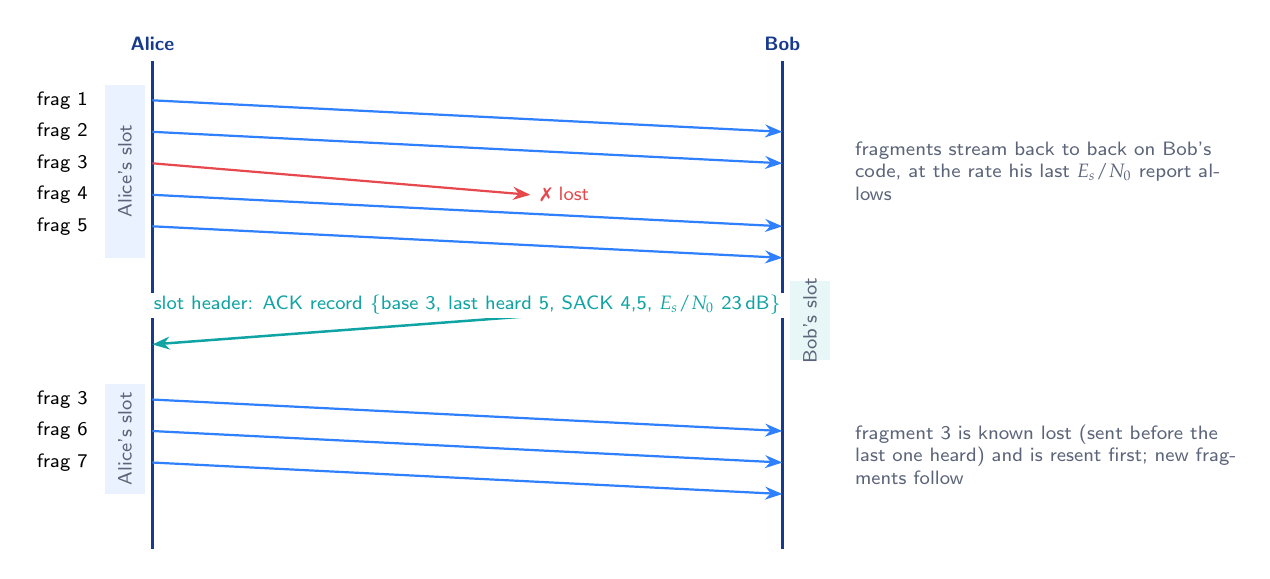
\begin{tikzpicture}[x=1mm,y=1mm]
  \draw[wldeep,line width=1pt] (0,0) node[above,lbl]{Alice} -- (0,-62);
  \draw[wldeep,line width=1pt] (80,0) node[above,lbl]{Bob} -- (80,-62);
  % Alice slot 1
  \fill[wlblue!10] (-6,-3) rectangle (-1,-25); \node[note,rotate=90] at (-3.5,-14) {Alice's slot};
  \foreach \k/\y in {1/-5,2/-9,3/-13,4/-17,5/-21}{
    \ifnum\k=3
      \draw[->,wlcoral,line width=0.8pt] (0,\y) -- (48,\y-4) node[right,font=\sffamily\scriptsize,text=wlcoral]{\ding{55} lost};
    \else
      \draw[->,wlblue,line width=0.8pt] (0,\y) -- (80,\y-4);
    \fi
    \node[font=\sffamily\scriptsize,anchor=east] at (-7,\y) {frag \k};
  }
  % Bob slot with ACK record
  \fill[wlteal!10] (81,-28) rectangle (86,-38); \node[note,rotate=90] at (83.5,-33) {Bob's slot};
  \draw[->,wlteal,line width=0.9pt] (80,-30) -- (0,-36);
  \node[font=\sffamily\scriptsize,text=wlteal,fill=white,inner sep=1pt] at (40,-31) {slot header: ACK record \{base 3, last heard 5, SACK 4,5, \EsNo\ 23\,dB\}};
  % Alice slot 2
  \fill[wlblue!10] (-6,-41) rectangle (-1,-55); \node[note,rotate=90] at (-3.5,-48) {Alice's slot};
  \foreach \k/\y in {3/-43,6/-47,7/-51}{
    \draw[->,wlblue,line width=0.8pt] (0,\y) -- (80,\y-4);
    \node[font=\sffamily\scriptsize,anchor=east] at (-7,\y) {frag \k};
  }
  \node[note,anchor=west,text width=48mm,align=left] at (88,-50) {fragment 3 is known lost (sent before the last one heard) and is resent first; new fragments follow};
  \node[note,anchor=west,text width=48mm,align=left] at (88,-14) {fragments stream back to back on Bob's code, at the rate his last \EsNo\ report allows};
\end{tikzpicture}
\caption{Selective-repeat ARQ under TD-CDMA: acknowledgements ride in the receiver's slot header.}
\label{fig:arq}
\end{figure}

A fragment that was sent before the fragment heard last and is still missing is known to be lost and
goes again in the sender's next slot (\cref{fig:arq}). A timeout resends whatever is in flight:
three cycles plus two hand-over times plus \SI{0.1}{s}, or $2.5\times$ the measured round-trip time plus
a cycle if that is longer. A large transfer streams in every slot, up to 496 fragments ahead of the
first unacknowledged one. Under spread ALOHA, the sender instead sets an ACK-request flag every half
second of airtime and pauses briefly so that the receiver can reply without being deafened.

\section{Adaptive modulation and coding}\label{sec:amc}
Every acknowledgement carries the \EsNo\ that the receiver measured, so the sender always knows the
quality of each link. The rung for each frame is chosen by the following rules.

\begin{algobox}{Algorithm 2: choosing the rung for a frame (\code{mac.py})}
\small
\begin{enumerate}[leftmargin=*,label=\arabic*.]
  \item Take the latest \EsNo\ report for the destination, corrected for the power the sender will
        use (\cref{sec:power}).
  \item Choose the fastest rung of \cref{tab:mcs} whose threshold the report meets.
  \item If recent windows (every 8 acknowledged frames under TD-CDMA) lost more than 20\,\% of their
        frames, step down one rung for \SI{10}{s}.
  \item For a message of one or two fragments, go two rungs lower (a lost frame costs a whole round
        trip), but never so low that one fragment no longer fits the sender's current slot.
  \item Group messages use the rung of the weakest member; acknowledgements, beacons and slot
        headers always use QPSK $\tfrac12$.
\end{enumerate}
\end{algobox}

Interference counts as noise in the reports. Under spread ALOHA, a second equal-power link on the
channel reduces the measured SNR to about 12--\SI{15}{dB}, and the link moves from uncoded 16-QAM to
16-QAM $\tfrac34$ or $\tfrac23$ rather than collapsing to QPSK.

\section{Priority handling}\label{sec:prio}
Each message belongs to one of four priority classes: \emph{control} (protocol and game-center
messages), \emph{urgent} (marked by the user with a lightning button), \emph{normal} (text) and \emph{bulk}
(photos, voice notes, files). When a slot is built, each destination's code serves its messages in
priority order, so an urgent text overtakes a \SI{10}{MB} transfer in the sender's very next slot.
Because texts are normal and media bulk, a photo sent just before a text usually arrives after it;
the application then places it by its send time (\cref{sec:chat}).

\section{Transmit power control}\label{sec:power}
Under spread ALOHA several stations transmit at once, and the \emph{near--far problem} appears: when
Alice talks at full power to Carol beside her, her signal swamps Bob's weak signal from across the
room at Dave, also beside her. Despreading leaves an interferer at its chip-level SNR, so every
decibel that Alice arrives above what Carol needs is a decibel of extra noise for Dave. TD-CDMA
removes the problem by construction, but power control is still useful there: it sets each slot's
level to what its weakest listener needs, so a station next to us arrives at about \SI{25}{dB}
instead of 40--\SI{50}{dB} and overdrives no receiver.

\begin{figure}[htbp]
\centering
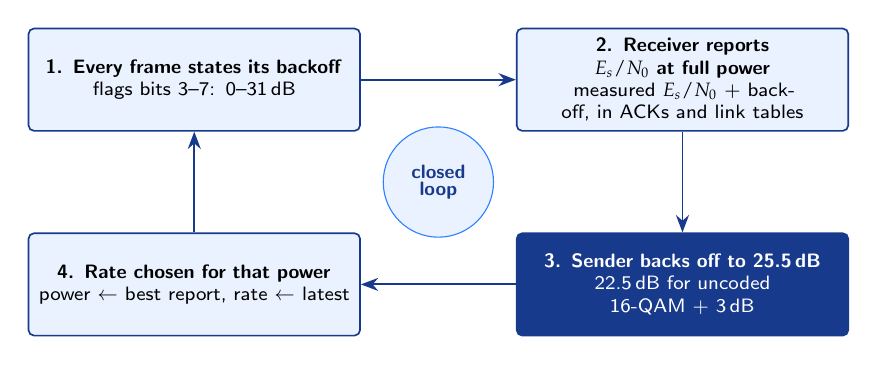
\begin{tikzpicture}[pc/.style={blk,minimum width=42mm,text width=40mm,minimum height=13mm,font=\sffamily\scriptsize}]
  \node[pc] (a) at (0,0) {\textbf{1. Every frame states its backoff}\\flags bits 3--7: 0--31\,dB};
  \node[pc] (b) at (62mm,0) {\textbf{2. Receiver reports \EsNo\ at full power}\\measured \EsNo\ + backoff, in ACKs and link tables};
  \node[pc,fill=wldeep,text=white] (c) at (62mm,-26mm) {\textbf{3. Sender backs off to 25.5\,dB}\\22.5\,dB for uncoded 16-QAM + 3\,dB};
  \node[pc] (d) at (0,-26mm) {\textbf{4. Rate chosen for that power}\\power $\leftarrow$ best report, rate $\leftarrow$ latest};
  \draw[flow] (a) -- (b); \draw[flow] (b) -- (c); \draw[flow] (c) -- (d); \draw[flow] (d) -- (a);
  \node[circle,draw=wlblue,fill=wllight,font=\sffamily\scriptsize\bfseries,text=wldeep,minimum size=14mm,align=center] at (31mm,-13mm) {closed\\[-2pt]loop};
\end{tikzpicture}
\caption{The closed transmit power-control loop.}\label{fig:pcloop}
\end{figure}

\Cref{fig:pcloop} shows the loop. Let $\hat\gamma_\text{full}$ be the receiver's \EsNo\ at full power and
$\Gamma=\SI{25.5}{dB}$ the target. The backoff is
\begin{equation}
  \beta=\min\!\left(30\,\mathrm{dB},\ \max\!\left(0,\ \hat\gamma_\text{full}-\Gamma-\delta_\text{outer}\right)\right),
\end{equation}
where $\delta_\text{outer}\in[0,12]$\,dB is raised by \SI{3}{dB} when a quiet link keeps losing frames
while backed off, and lowered by \SI{1}{dB} per \SI{30}{s} without losses. Power goes up at once but
down only in steps of at least \SI{2}{dB}. Crucially, the reports are SINR values that drop while
someone else is on the air. Power therefore follows the \emph{best} recent report (which tracks the
path), while the rate follows the \emph{latest} one (which includes interference). A burst of
interference then lowers the rate rather than raising the power, which would only start a power race
between stations. The target of \SI{25.5}{dB} removes only power that the link cannot use: a lower
target such as \SI{17}{dB} protects weak neighbours more, but forces every strong link onto slower
coded rungs, which costs airtime and receiver CPU at every station.

%% =====================================================================
\chapter{TD-CDMA Medium Access and Relaying}\label{ch:tdcdma}
%% =====================================================================
TD-CDMA (\code{tdma.py}) organises the stations into a repeating \emph{cycle} of time slots. In its
own slot a station is the only transmitter on the air, and it uses code division to reach every other
station at once. This chapter describes the cycle, how stations agree on it without a central
controller, how slots are timed to the radio sample, and how messages reach stations that cannot
hear each other.

\section{The cycle}\label{sec:cycle}
\Cref{fig:cycle} is drawn to scale for a busy cycle with four stations in which Alice sends a photo to
Bob and a voice note to Carol at the same time. Every slot begins with its owner's \emph{slot header}
on the broadcast code at QPSK $\tfrac12$ (4.6--\SI{9.6}{ms}). From the same chip, the owner's frames for
each destination start on that destination's code. A slot with queued data grows to a whole number
of frames close to \SI{100}{ms} (at most \SI{250}{ms}); an idle slot is \SI{15}{ms}; the \emph{join slot}
at the end of the cycle (\SI{11.5}{ms}) is where newcomers announce themselves. A guard of \SI{0.5}{ms}
separates slots; the plan is counted in ticks of \SI{0.25}{ms}.

\begin{figure}[htbp]
\centering
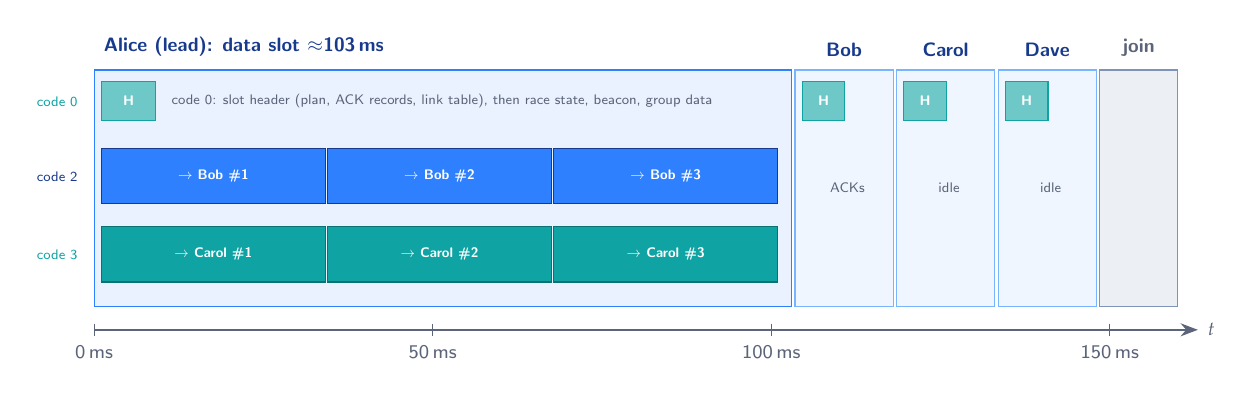
\begin{tikzpicture}[x=0.86mm,y=1mm]
  % slots: Alice 103 ms, Bob 15, Carol 15, Dave 15, join 11.5  (scale 1 ms = 0.86 mm)
  \fill[wlblue!10] (0,0) rectangle (103,30);   \draw[wlblue] (0,0) rectangle (103,30);
  \fill[wlsky!12] (103.5,0) rectangle (118,30); \draw[wlsky] (103.5,0) rectangle (118,30);
  \fill[wlsky!12] (118.5,0) rectangle (133,30); \draw[wlsky] (118.5,0) rectangle (133,30);
  \fill[wlsky!12] (133.5,0) rectangle (148,30); \draw[wlsky] (133.5,0) rectangle (148,30);
  \fill[wlsteel!15] (148.5,0) rectangle (160,30); \draw[wlsteel] (148.5,0) rectangle (160,30);
  \node[lbl,anchor=south west] at (0,30.5) {Alice (lead): data slot $\approx$103\,ms};
  \foreach \x/\n in {110.75/Bob,125.75/Carol,140.75/Dave}{\node[lbl,anchor=south] at (\x,30.5) {\n};}
  \node[lbl,anchor=south,text=wlgrey] at (154.25,30.5) {join};
  % Alice's lanes
  \node[draw=wlteal,fill=wlteal!60,font=\sffamily\tiny\bfseries,text=white,minimum height=5mm,minimum width=6.9mm,inner sep=0,anchor=south west] at (1,23.5) {H};
  \node[font=\sffamily\tiny,anchor=west,text=wlgrey] at (10,26) {code 0: slot header (plan, ACK records, link table), then race state, beacon, group data};
  \foreach \i in {0,1,2}{
    \node[draw=wldeep,fill=wlblue,font=\sffamily\tiny\bfseries,text=white,minimum height=7mm,minimum width=28.4mm,inner sep=0,anchor=south west] at (1+\i*33.4,13) {$\to$ Bob \#\the\numexpr\i+1\relax};
    \node[draw=wlteal!70!black,fill=wlteal,font=\sffamily\tiny\bfseries,text=white,minimum height=7mm,minimum width=28.4mm,inner sep=0,anchor=south west] at (1+\i*33.4,3) {$\to$ Carol \#\the\numexpr\i+1\relax};
  }
  \node[font=\sffamily\tiny,text=wlblue,anchor=west] at (101.5,16.5) {};
  % idle slots
  \foreach \x/\t in {104.5/ACKs,119.5/idle,134.5/idle}{
    \node[draw=wlteal,fill=wlteal!60,font=\sffamily\tiny\bfseries,text=white,minimum height=5mm,minimum width=5.4mm,inner sep=0,anchor=south west] at (\x,23.5) {H};
    \node[font=\sffamily\tiny,text=wlgrey] at (\x+6.75,15) {\t};
  }
  % code labels
  \node[font=\sffamily\tiny,text=wldeep,anchor=east] at (-1,16.5) {code 2};
  \node[font=\sffamily\tiny,text=wlteal,anchor=east] at (-1,6.5) {code 3};
  \node[font=\sffamily\tiny,text=wlteal,anchor=east] at (-1,26) {code 0};
  % axis
  \draw[->,wlgrey,line width=0.6pt] (0,-3) -- (163,-3) node[right,note]{$t$};
  \foreach \x/\l in {0/0,50/50,100/100,150/150}{\draw[wlgrey] (\x,-2.2) -- (\x,-3.8) node[below,note]{\l\,ms};}
\end{tikzpicture}
\caption{One TD-CDMA cycle drawn to scale: Alice's data slot carries frames for Bob (code~2) and Carol
(code~3) simultaneously, followed by the idle slots of Bob, Carol and Dave and the join slot.}
\label{fig:cycle}
\end{figure}

The cycle length adapts to demand (\cref{fig:cyclelen}). With every station idle it is about
\SI{100}{ms}: the spare time is spread over the slots, which keeps the header rate at ten per station
per second and leaves room in an idle slot for a beacon or a short message without changing the plan.
With every station sending, it grows to 213.5, 333.5 and \SI{415.5}{ms} for two, three and four
stations. A cycle longer than \SI{700}{ms} has its data slots shortened in proportion.

\begin{figure}[htbp]
\centering
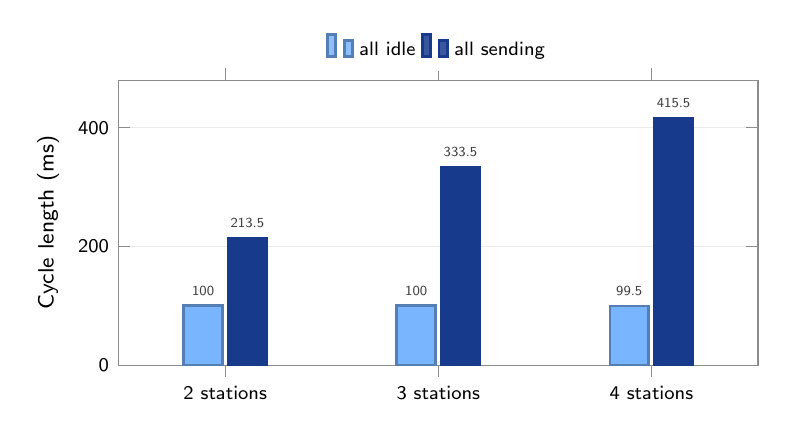
\begin{tikzpicture}
\begin{axis}[wlbar,width=0.8\linewidth,height=52mm,ymin=0,ymax=480,bar width=14pt,
  symbolic x coords={2 stations,3 stations,4 stations},xtick=data,ylabel={Cycle length (ms)},
  legend style={at={(0.5,1.03)},anchor=south,legend columns=2},enlarge x limits=0.25]
\addplot[fill=wlsky,draw=wlsky!70!black] coordinates {(2 stations,100)(3 stations,100)(4 stations,99.5)};
\addplot[fill=wldeep,draw=wldeep] coordinates {(2 stations,213.5)(3 stations,333.5)(4 stations,415.5)};
\legend{all idle,all sending}
\end{axis}
\end{tikzpicture}
\caption{Measured cycle length (numpy simulator) with all stations idle and with all stations sending.}
\label{fig:cyclelen}
\end{figure}

\section{Distributed control: lead, join, plan changes and takeover}\label{sec:control}
There is no fixed master; the network organises itself through the slot headers.
\begin{description}[style=nextline,leftmargin=0pt,font=\sffamily\bfseries\color{wldeep}]
  \item[The lead.] The first station on the air leads: its header opens each cycle and carries the
    cycle number and the slot plan. A starting station listens for \SI{1.2}{s} plus \SI{0.25}{s} per
    address above 1, so among stations switched on together the lowest address leads. A station
    that hears a lead joins it. When two networks meet, the lower lead address wins.
  \item[Joining.] Before it knows its own timing offset, a newcomer transmits only quiet
    \emph{probes}: its header on its own code (which nobody despreads), \SI{20}{dB} down. Once it has
    measured its offset it sends a join request in the join slot, at a random point of its first
    \SI{4}{ms} and in a random half of the cycles, so two newcomers rarely collide. The lead adds it to
    the plan.
  \item[Plan changes.] Joins, departures and changes of airtime are announced in the lead's header
    at least \SI{1}{s} and four cycles before they take effect, one change at a time, and every lead
    header repeats the plan in force. A station that has not heard the plan recently enough
    \emph{holds its slot} rather than transmit by a stale plan. The \SI{1}{s} horizon covers the 0.2--\SI{0.6}{s}
    latency between building a burst and its leaving the antenna.
  \item[Leaving and takeover.] A station whose headers stop for six cycles and \SI{1.5}{s} loses its
    slot. If the lead falls silent for two cycles, the next lowest address takes over, but only if it
    still hears other stations and none of them reports hearing the lead; otherwise it is the one cut
    off, and it marks its header \emph{lead unheard} while others repeat the plan for it. In our
    GNU Radio test with emulated ANTSDRs, a killed lead was replaced after \SI{0.71}{s} and the transfer
    in progress continued.
\end{description}

\section{Timing in radio samples}\label{sec:timing}
The PC's clock and its buffering jitter (tens of milliseconds) are useless for slots whose guard is
\SI{0.5}{ms}. WaveLink therefore keeps all timing in the sample counters of the radios, where it is exact
(\cref{fig:timing}).

\begin{figure}[htbp]
\centering
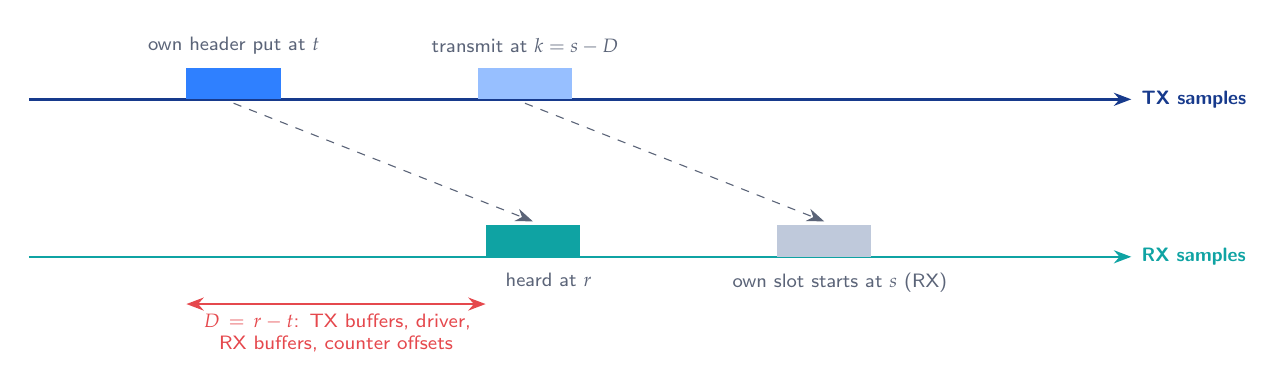
\begin{tikzpicture}[x=1mm,y=1mm]
  \draw[->,wldeep,line width=0.9pt] (0,20) -- (140,20) node[right,lbl]{TX samples};
  \draw[->,wlteal,line width=0.9pt] (0,0) -- (140,0) node[right,lbl,text=wlteal]{RX samples};
  \fill[wlblue] (20,20) rectangle (32,24); \node[note,anchor=south] at (26,24.5) {own header put at $t$};
  \fill[wlteal] (58,0) rectangle (70,4); \node[note,anchor=north] at (66,-0.8) {heard at $r$};
  \draw[->,wlgrey,dashed] (26,19.5) -- (64,4.5);
  \draw[<->,wlcoral,line width=0.8pt] (20,-6) -- node[below,font=\sffamily\scriptsize,text=wlcoral,text width=40mm,align=center]{$D=r-t$: TX buffers, driver, RX buffers, counter offsets} (58,-6);
  \fill[wlsteel!50] (95,0) rectangle (107,4); \node[note,anchor=north] at (103,-0.8) {own slot starts at $s$ (RX)};
  \fill[wlblue!50] (57,20) rectangle (69,24); \node[note,anchor=south] at (63,24.5) {transmit at $k=s-D$};
  \draw[->,wlgrey,dashed] (63,19.5) -- (101,4.5);
\end{tikzpicture}
\caption{The transmit-to-receive offset $D$ maps a desired receive-side slot start onto the transmit stream.}
\label{fig:timing}
\end{figure}

Transmitter and receiver of one ANTSDR run from one sample clock, and a station hears its own
transmitter through the antenna leakage. Every slot header carries the transmit sample index $t$ at
which it was placed in the stream; when the station receives its own header at receive index $r$, it
learns its \emph{TX$\to$RX offset}
\begin{equation}
  D=r-t .
\end{equation}
$D$ contains the transmit buffers, the driver, the kernel and receive buffers and the arbitrary start
of the two counters, none of which needs to be known individually. It is constant to the sample
until a transmit underrun or a lost receive buffer, and is re-measured in every slot.

A follower converts the lead's header, heard at receive index $j$, into the start of cycle $n$ in its
own receive count, $c_n=j-(\text{lead's slot start}+\tfrac12\,\text{guard})$. Its own slot then starts
at $s=c_n+\text{own slot start}+\tfrac12\,\text{guard}$ in receive samples, and it transmits at
\begin{equation}
  k=s-D \quad\text{(transmit samples)}.
\end{equation}
The Burst Combiner block places the burst exactly at chip $k$. Clock drift does not accumulate: every
lead header re-anchors the followers, which also estimate their clock ratio to the lead (shown in ppm
on the dashboard) to bridge missed headers. The \SI{0.5}{ms} guard covers the RRC tails, detection
error (about 0.25 sample RMS), drift between headers (\SI{50}{ppm} over a \SI{400}{ms} cycle is
\SI{20}{\micro s}) and propagation delay. If a station cannot hear itself, the others steer it: every
header reports, for each station heard, how many samples off its header arrived, and the station
corrects $D$ by 0.7 times the median report.

\section{Slot-aware receiver search}\label{sec:search}
Because bursts can only start at known instants, the receiver searches for preambles only where a
burst can begin: around every other station's slot start ($\pm\SI{0.27}{ms}$), immediately after every
burst it has found (the next follows back to back), and across the join slot on the broadcast code.
Every eighth cycle, while the lead's header is missing, and for \SI{1.5}{s} after a possible timing slip
it searches everywhere. This reduced the search to 9.5--16\,\% of the samples and, in the simulator,
the receive CPU of three idle stations from 3.2 to \SI{1.2}{s} per second of air.

\section{One-hop relaying}\label{sec:relay}
Every slot header carries a \emph{link table}: the \EsNo\ (at full power) at which its station hears every
other station. From these tables every station knows who hears whom. When a destination does not hear
us, or messages to it keep timing out, and a station with relaying enabled hears both ends at
\SI{7}{dB} or more, messages are routed through that station (\cref{fig:relay}).

\begin{figure}[htbp]
\centering
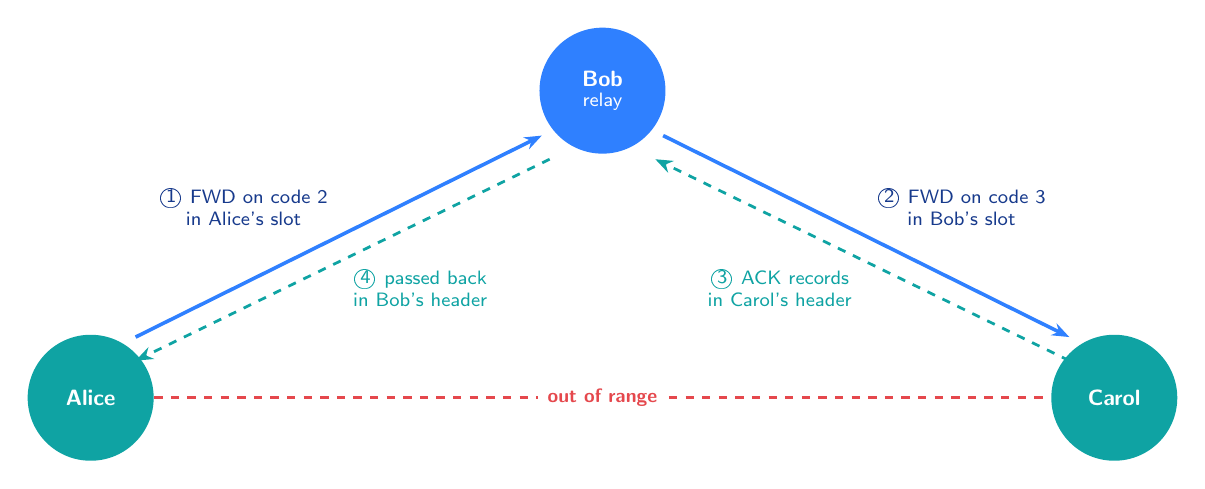
\begin{tikzpicture}[x=1.3mm,y=1.3mm]
  \node[station,fill=wlteal,minimum size=16mm,font=\sffamily\footnotesize\bfseries] (A) at (0,0) {Alice};
  \node[station,minimum size=16mm,font=\sffamily\footnotesize\bfseries] (B) at (50,30) {Bob\\[-2pt]{\scriptsize\mdseries relay}};
  \node[station,fill=wlteal,minimum size=16mm,font=\sffamily\footnotesize\bfseries] (C) at (100,0) {Carol};
  \draw[wlcoral,dashed,line width=1pt] (A) -- node[pos=0.5,fill=white,font=\sffamily\scriptsize\bfseries,text=wlcoral]{out of range} (C);
  \draw[->,wlblue,line width=1.3pt] ([yshift=2mm]A.north east) -- node[above left,font=\sffamily\scriptsize,text=wldeep,align=center]{\textcircled{\scriptsize 1} FWD on code 2\\in Alice's slot} ([xshift=-2mm]B.south west);
  \draw[->,wlblue,line width=1.3pt] ([xshift=2mm]B.south east) -- node[above right,font=\sffamily\scriptsize,text=wldeep,align=center]{\textcircled{\scriptsize 2} FWD on code 3\\in Bob's slot} ([yshift=2mm]C.north west);
  \draw[->,wlteal,dashed,line width=1pt] ([yshift=-1mm]C.north west) -- node[below left,font=\sffamily\scriptsize,text=wlteal,align=center]{\textcircled{\scriptsize 3} ACK records\\in Carol's header} ([xshift=1mm,yshift=-3mm]B.south east);
  \draw[->,wlteal,dashed,line width=1pt] ([xshift=-1mm,yshift=-3mm]B.south west) -- node[below right,font=\sffamily\scriptsize,text=wlteal,align=center]{\textcircled{\scriptsize 4} passed back\\in Bob's header} ([yshift=-1mm]A.north east);
\end{tikzpicture}
\caption{One-hop relaying from Alice to Carol through Bob. Every station still despreads only its own code and code~0.}
\label{fig:relay}
\end{figure}

The relay passes on FWD frames in its own slot, at the rate of the last hop. At most 256 frames per
destination wait at the relay, and each fragment is queued once: a copy repeated by the sender while
the first is still waiting is dropped. Carol's ACK records reach Bob in her header and are passed back
to Alice in Bob's next header. A route returns to the direct path after the direct link has been good
(at least \SI{5}{dB}, no timeouts) for \SI{5}{s}. Members that hear the lead also repeat the lead's plan
for stations that cannot hear it, so a hidden station keeps time even with relaying switched off.
Names and profile photos of stations reachable only through a relay are passed on as well.

We preferred this over two alternatives. A hub through which all traffic passes would double the
airtime of every message and stop the network when it fails; a ring would add up to three hops.
One-hop relaying costs extra airtime only for the pairs that need it.

\section{Messages of any size}\label{sec:anysize}
The same wrappers carry every message, from a short text to a \SI{64}{MB} file (\cref{fig:pipeline}).
The application shrinks the content first (zlib for text and compressible files, WebP for photos, Opus
for voice notes), wraps it in one envelope (paying the metadata and the 28 bytes of AES-GCM once),
and the link layer cuts it into fragments, each a DATA frame with 14 bytes of overhead and its own
burst with 96 symbols of preamble and header. A short message fits into the sender's next slot: a text
from Alice reaches Bob in about \SI{75}{ms}. A large transfer asks for a data slot of whole frames close
to \SI{100}{ms}, granted about \SI{1.4}{s} later (plan changes are announced \SI{1}{s} ahead), after which
three full frames go out per cycle: \SI{187}{kb/s} with two stations and \SI{152}{kb/s} with four.

\begin{figure}[htbp]
\centering
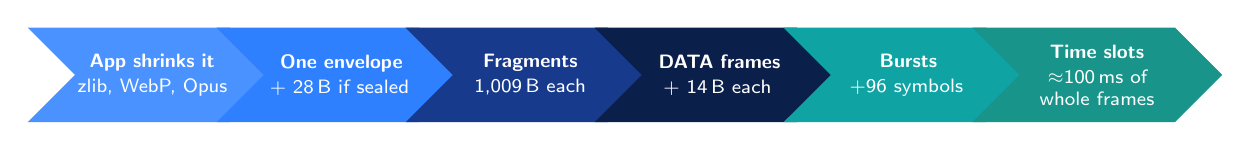
\begin{tikzpicture}[chev/.style={shape=signal,signal to=east,signal from=west,draw=none,minimum height=12mm,
    minimum width=23.5mm,text width=19mm,font=\sffamily\scriptsize,text=white,align=center,inner sep=1pt}]
  \foreach \i/\a/\b/\c in {0/App shrinks it/{zlib, WebP, Opus}/wlblue!65!wlsky,1/One envelope/{+ 28\,B if sealed}/wlblue,
     2/Fragments/{1,009\,B each}/wldeep,3/DATA frames/{+ 14\,B each}/wlnavy,4/Bursts/{+96 symbols}/wlteal,
     5/Time slots/{$\approx$100\,ms of whole frames}/wlmint!70!black}
    \node[chev,fill=\c] at (\i*24mm,0) {\textbf{\a}\\[1pt]\b};
\end{tikzpicture}
\caption{The packetization pipeline shared by every message.}\label{fig:pipeline}
\end{figure}

\Cref{fig:delivery} shows typical delivery times for representative messages, from a model of the slot
schedule of \code{tdma.py} that agrees with the simulator running the project's code to within
\SI{0.06}{s} for short messages and 15\,\% for long ones. Note the logarithmic axis: delivery time spans
more than three orders of magnitude, and with four stations a two-fragment message already waits for
its sender's slot to grow.

\begin{figure}[htbp]
\centering
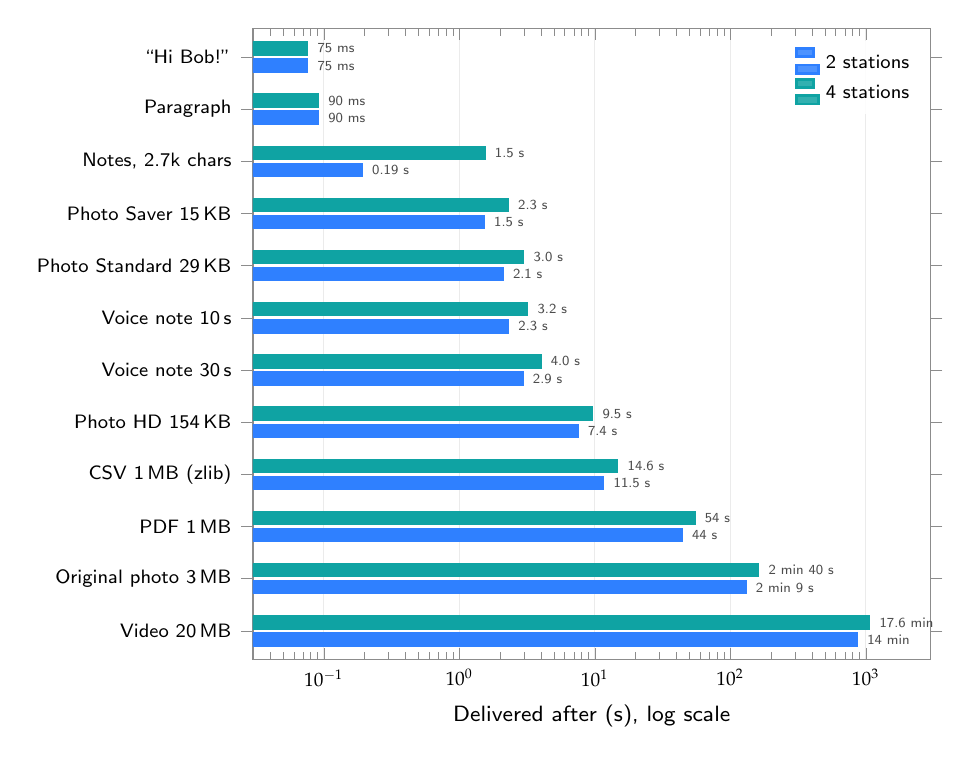
\begin{tikzpicture}
\begin{axis}[wl,xbar,xmode=log,log basis x=10,width=0.84\linewidth,height=96mm,
  xmin=0.03,xmax=3000,bar width=4.2pt,
  symbolic y coords={vid,orig,pdf,csv,hd,v30,v10,std,saver,notes,para,hi},log origin=infty,
  ytick={vid,orig,pdf,csv,hd,v30,v10,std,saver,notes,para,hi},yticklabels={Video 20\,MB,Original photo 3\,MB,PDF 1\,MB,{CSV 1\,MB (zlib)},Photo HD 154\,KB,Voice note 30\,s,Voice note 10\,s,Photo Standard 29\,KB,Photo Saver 15\,KB,{Notes, 2.7k chars},Paragraph,``Hi Bob!''},y dir=normal,xlabel={Delivered after (s), log scale},
  legend style={at={(0.99,0.98)},anchor=north east},xmajorgrids,ymajorgrids=false,
  nodes near coords,every node near coord/.append style={font=\sffamily\tiny,text=black!70,anchor=west},
  point meta=explicit symbolic,enlarge y limits=0.05]
\addplot[fill=wlblue,draw=wlblue] coordinates {
 (0.075,hi)[75 ms] (0.09,para)[90 ms] (0.19,notes)[0.19 s] (1.51,saver)[1.5 s]
 (2.08,std)[2.1 s] (2.28,v10)[2.3 s] (2.92,v30)[2.9 s] (7.44,hd)[7.4 s]
 (11.5,csv)[11.5 s] (43.6,pdf)[44 s] (129,orig)[2 min 9 s] (856,vid)[14 min]};
\addplot[fill=wlteal,draw=wlteal] coordinates {
 (0.075,hi)[75 ms] (0.09,para)[90 ms] (1.53,notes)[1.5 s] (2.27,saver)[2.3 s]
 (2.95,std)[3.0 s] (3.16,v10)[3.2 s] (3.95,v30)[4.0 s] (9.52,hd)[9.5 s]
 (14.6,csv)[14.6 s] (54.1,pdf)[54 s] (160,orig)[2 min 40 s] (1055,vid)[17.6 min]};
\legend{2 stations,4 stations}
\end{axis}
\end{tikzpicture}
\caption{Typical delivery times from Alice to Bob on a link running uncoded 16-QAM, with two and with
four stations (model of the TD-CDMA schedule, calibrated against the simulator).}\label{fig:delivery}
\end{figure}
%% =====================================================================
\chapter{Application Layer}\label{ch:app}
%% =====================================================================
The application (\code{node.py}, \code{games/} and \code{web/}) turns the radio network into a
product: a messenger and a game center that run in any browser, served by the station itself over
plain HTTP with Server-Sent Events for live updates. The web server uses only the Python standard
library and the user interface loads nothing from the internet, so a station works fully offline.

\section{Message envelope and compression}
Every message is one \emph{envelope}:
\begin{center}

\begin{tikzpicture}[f/.style={draw=white,line width=1pt,minimum height=8mm,font=\sffamily\scriptsize,
  text=white,align=center,anchor=west,inner sep=2pt}]
  \node[f,fill=wldeep,minimum width=17mm] (a) at (0,0) {crypto byte};
  \node[f,fill=wldeep,minimum width=19mm] (b) at (a.east) {meta length};
  \node[f,fill=wlblue,minimum width=50mm] (c) at (b.east) {meta JSON: kind, uid, time, group, name, type};
  \node[f,fill=wlsteel,minimum width=36mm] (d) at (c.east) {body};
\end{tikzpicture}
\end{center}
The \emph{kind} is one of \code{text}, \code{image}, \code{audio}, \code{file}, \code{game},
\code{rcpt} (read receipt), \code{gc} (game center), \code{prof} (profile picture) or \code{ctl}
(cancel and stop). Text, and files that compress, are zlib-compressed before sending: a file over
\SI{2}{KB} is compressed only if its first \SI{256}{KB} shrink below 90\,\% at level~1 and the whole file
below 95\,\%, so already-compressed media are never compressed twice. The UI shows an airtime estimate
at the link's current rate before a large file is sent.

\section{Encryption}\label{sec:crypto}
With a shared passphrase, every envelope is sealed with AES-256 in Galois/Counter Mode~\cite{gcm}. The
256-bit key is derived from the passphrase with scrypt~\cite{scrypt}, each message uses a fresh random
96-bit nonce, and the pair (source, destination) is passed as \emph{associated data}: it is
authenticated but not encrypted, so a message captured and replayed towards another station fails
authentication. The cost is 28 bytes per message (a 12-byte nonce and a 16-byte tag), paid once per
envelope rather than per fragment. Beacons advertise a short key identifier, and the UI warns when a
peer uses a different key; its messages then cannot be opened.

\section{The chat}\label{sec:chat}
The chat offers one-to-one conversations and an \emph{Everyone} group (\cref{fig:chat}). Its delivery
indicators map directly onto link-layer events (\cref{tab:ticks}).

\begin{figure}[htbp]
\centering
\begin{subfigure}[b]{0.585\linewidth}\centering
\includegraphics[width=\linewidth]{figures/chat_sending.jpg}
\caption{Sending a photo, a voice note and a 1.4\,MB file}
\end{subfigure}\hfill
\begin{subfigure}[b]{0.395\linewidth}\centering
\includegraphics[width=\linewidth,trim=445 130 443 145,clip]{figures/photo_sheet.jpg}
\caption{Choosing the photo quality}
\end{subfigure}
\caption{The WaveLink chat (screenshots of the running application). The header shows the live link:
code, \EbNo, carrier offset and the current rung (here uncoded 16-QAM, 258\,kb/s).}\label{fig:chat}
\end{figure}

\begin{table}[htbp]
\centering\small
\caption{Message status indicators and the events behind them.}\label{tab:ticks}
\begin{tabular}{@{}cl@{}}
\toprule
\textbf{Indicator} & \textbf{Meaning}\\
\midrule
clock & queued at the sender\\
\ding{51} & on the air\\
\ding{51}\ding{51} & acknowledged: every fragment confirmed by an ACK record (group: by every member)\\
\emph{2/3} \ding{51} & group message acknowledged by some members so far\\
\textcolor{wlblue}{\ding{51}\ding{51}} & read: the recipient opened the chat (read receipt)\\
! / \ding{198} & failed after retries / cancelled by either end\\
\bottomrule
\end{tabular}
\end{table}

\paragraph{Media at a chosen quality.} Picking a photo or finishing a voice note opens a sheet that
has already produced every version, with its size and time on air at the link's current rate. Photos
are re-encoded in the browser as WebP at 480\,px (Saver), 640\,px (Standard) or 1280\,px (HD), or sent
as the original. Voice notes of up to \SI{30}{s} are re-encoded with the browser's Opus
encoder~\cite{opus} at 12 or \SI{24}{kb/s} and packed into WebM by a small muxer of our own.

\paragraph{Messages in the order they were sent.} Because texts overtake bulk media on the air, a photo
sent just before a text may arrive after it. Every message therefore carries its send time on the
sender's clock, and each station estimates every other station's clock offset as
\begin{equation}
  \hat\theta=\min_{\text{last 5 min}}\left(t_\text{arrival}-t_\text{sent}\right),
\end{equation}
which equals the true offset plus the shortest delivery time (tens of milliseconds, up to about one
cycle under TD-CDMA). A received message is placed at its send time converted to the local clock, and
slides into place if it arrived late, marked ``late'' when the delay exceeds \SI{4}{s}.

\paragraph{Profiles over the air.} Names and a short profile-picture tag (a hash of the photo) travel in
the beacons. A station that sees an unknown hash requests the photo once; it therefore crosses the air
once per pair of stations, and again only when it changes. Eight colour themes, chat wallpapers with an
editor, sound effects and synthesised background music complete the experience.

\section{Game center}\label{sec:games}
The game center hosts two games for two to four stations (\cref{fig:games}). They illustrate two
opposite traffic patterns: UNO needs reliable, ordered, secret messages; the race needs frequent,
small, loss-tolerant updates.

\begin{figure}[htbp]
\centering
\begin{subfigure}[b]{0.49\linewidth}\centering
\includegraphics[width=\linewidth]{figures/uno.jpg}
\caption{UNO, three players: each screen shows only its own hand}
\end{subfigure}\hfill
\begin{subfigure}[b]{0.49\linewidth}\centering
\includegraphics[width=\linewidth]{figures/race.jpg}
\caption{Gold Code GP, a real-time street race with pickups}
\end{subfigure}
\caption{The game center running over the radio network (screenshots).}\label{fig:games}
\end{figure}

\subsection{UNO: the host's station as referee}
The host's station shuffles, deals and keeps every hand. Players send \emph{intents} (``play card 37
as blue'', ``draw'') as reliable control-priority messages; the host's rules engine checks them and
sends each player a fresh \emph{view} containing only that player's hand and the others' card counts,
so a hand never leaves its owner's screen. A turn lasts at most \SI{30}{s}, after which the host plays a
timeout move. If the host leaves the air, the next player in seat order takes over: every view carries
a hidden copy of the table (kept in the station, never shown in the browser), and a host number
carried in every message lets an old host that returns recognise that it has been replaced. The rules
engine was verified with 300 random games.

\subsection{Gold Code GP: every station drives its own car}
The race track and city are generated from a shared random seed, so nothing but the seed crosses the
air. Each browser runs its own car's physics at 120 steps per second and posts the state to its
station 20 times a second. The station places the newest state in its own slot as an unacknowledged
datagram on the broadcast code: 28 bytes, plus 13 bytes per game event; with one event the frame is
52 bytes and \SI{7.9}{ms} at QPSK $\tfrac12$. Events (a missile fired, a mine dropped, a hit) are repeated
in the next four packets so that a single lost packet loses nothing. A hit is decided by the
\emph{victim's} station, which knows exactly where its own car was. Other cars are drawn by dead
reckoning along the track, and clocks are synchronised with datagram pings that keep the sample with
the shortest round trip.

\section{Radio dashboard}\label{sec:dash}
The graphical dashboard (\cref{fig:dash}), a bonus feature of the brief, exposes everything the radio
knows, live: the last frame's rung, symbol and chip SNR, \EbNo, carrier offset and preamble metric;
frames delivered, CRC-32 drops, retransmissions and LDPC iterations; the TD-CDMA plan, the lead, the
measured TX$\to$RX offset $D$, the clock against the lead in ppm, late bursts and where the receiver is
searching; the relay switch and routes; and the constellation and spectrum of the last burst. It opens
over the chat or over a running game.

\begin{figure}[!htbp]
\centering
\includegraphics[width=0.8\linewidth]{figures/uno_radio.jpg}
\caption{The radio dashboard open over a game of UNO (screenshot).}\label{fig:dash}
\end{figure}

%% =====================================================================
\chapter{Implementation and Verification}\label{ch:impl}
%% =====================================================================

\section{Development approach}
Laboratory time with the shared ANTSDRs was limited, so the team followed a simulation-first approach
in which every layer could be developed and tested without radios, and in which each step towards the
hardware replaced one simulated component with the real one (\cref{fig:envs}).

\begin{figure}[htbp]
\centering
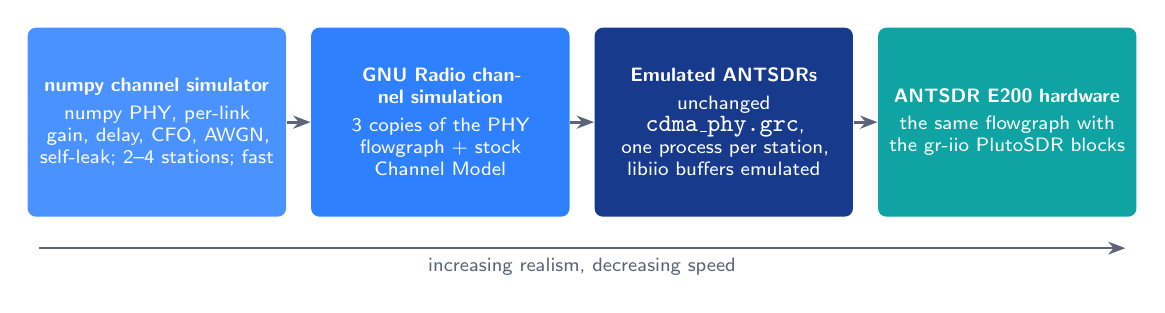
\begin{tikzpicture}[env/.style={draw=none,rounded corners=3pt,minimum height=24mm,text width=30mm,
  align=center,font=\sffamily\scriptsize,text=white,inner sep=4pt}]
  \node[env,fill=wlblue!65!wlsky] (e1) at (0,0) {\textbf{numpy channel simulator}\\[2pt]numpy PHY, per-link gain, delay, CFO, AWGN, self-leak; 2--4 stations; fast};
  \node[env,fill=wlblue] (e2) at (36mm,0) {\textbf{GNU Radio channel simulation}\\[2pt]3 copies of the PHY flowgraph + stock Channel Model};
  \node[env,fill=wldeep] (e3) at (72mm,0) {\textbf{Emulated ANTSDRs}\\[2pt]unchanged \code{cdma\_phy.grc}, one process per station, libiio buffers emulated};
  \node[env,fill=wlteal] (e4) at (108mm,0) {\textbf{ANTSDR E200 hardware}\\[2pt]the same flowgraph with the gr-iio PlutoSDR blocks};
  \foreach \a/\b in {e1/e2,e2/e3,e3/e4} \draw[->,line width=1.2pt,wlgrey] (\a) -- (\b);
  \draw[->,wlgrey,line width=0.6pt] (-15mm,-16mm) -- node[below,note]{increasing realism, decreasing speed} (123mm,-16mm);
\end{tikzpicture}
\caption{The four environments in which WaveLink runs. Each step replaces one simulated part with the real one.}
\label{fig:envs}
\end{figure}

\begin{description}[style=nextline,leftmargin=0pt,font=\sffamily\bfseries\color{wldeep}]
  \item[numpy channel simulator.] Up to four stations in one process, each with the numpy PHY. Every
    link has its own gain, delay (up to \SI{100}{\micro s}), carrier offset and noise; a station hears its
    own transmitter at a configurable level (\SI{25}{dB} above the others, as on the ANTSDRs). The
    simulated clock lets throughput be measured correctly even when the PC runs slower than real time.
  \item[GNU Radio channel simulation.] In \code{cdma\_phy\_sim.grc}, three copies of the station PHY are summed through the stock
    Channel Model block and run in GNU Radio at \SI{1}{MS/s}, because the three Python blocks share one
    interpreter.
  \item[Emulated ANTSDRs.] Each station is the unchanged application on the unchanged
    \code{cdma\_phy.grc}, in its own process, with only the two PlutoSDR blocks replaced by stand-ins
    with the same interface. The sink takes whole \code{tx\_buffer} buffers into a queue of four
    (libiio's default) drained at \SI{4}{MS/s}; the source delivers whole \num{32768}-sample buffers; both
    clip at full scale; an empty transmit queue sends zeros (underrun) and receive buffers not fetched
    in time are lost (overflow). A separate ``air'' process applies per-link gain, delay, phase and
    LO offset, the \SI{25}{dB} self-leak, noise, clock errors, interference and cut links.
  \item[Hardware.] The same flowgraph with the gr-iio blocks. The mid-evaluation simplex link used the
    \code{tx} and \code{rx} tools with a minimal GNU Radio graph.
\end{description}

The emulated ANTSDRs proved their worth: nine timing bugs appeared there and nowhere else, among them
a hidden station's join, a newcomer's first join request, bursts after a transmit underrun, slots held
while a slot grew, a restart mistaken for a duplicate address and two stations compiling the flowgraph
at once. All were fixed.

\section{Test suites}
\Cref{tab:tests} lists the automated test suites. Every result quoted in \cref{ch:results} comes from
one of them.

\begin{table}[htbp]
\centering\small
\caption{Automated test suites and their results.}\label{tab:tests}
\begin{tabularx}{\linewidth}{@{}>{\ttfamily\footnotesize}p{35mm}L>{\raggedright\arraybackslash}p{28mm}@{}}
\toprule
\textrm{\textbf{Suite}} & \textbf{What it checks} & \textbf{Result}\\
\midrule
test\_ldpc & Encoder at all 51 lifting sizes, rate matching, AWGN curves, Golay & all pass\\
test\_modem, test\_profiles & PHY impairments, false alarms, multi-user, SNR sweeps, decode cost & all pass\\
test\_grc\_flowgraph & The real flowgraph in GNU Radio: every rung, unicast and broadcast, 3 senders & 10/10, 3/3 frames\\
test\_grc\_cores & The flowgraph's Python cores with imitated stock blocks; numpy--GRC interoperability & all pass\\
test\_tdma\_phy & Bursts on exact samples, receive indices, $D$ under drift, underruns & 19/19\\
test\_edge & 17 TD-CDMA edge-case scenarios on the simulated air & 93/93 checks\\
test\_fake\_antsdr & 12 scenarios: full app on \code{cdma\_phy.grc} with emulated ANTSDRs & 55/58 checks\\
test\_power & Power-control loop, flowgraph power tags, near--far with and without control & 18/18\\
test\_uno, test\_games & UNO rules (300 random games); game center over the simulated air & all pass\\
ui\_features, ui\_games & Browser UI driven by Playwright on every station's page & 65/65; games played\\
\bottomrule
\end{tabularx}
\end{table}

\section{Hardware bring-up procedure}
The procedure prepared for the laboratory sessions follows the same ladder: verify that the PC reaches
the device (\code{iio\_info}), run a loop-back self-test of the GNU Radio installation, compile the
flowgraph, then run the mid-evaluation simplex link:
\begin{lstlisting}[language=bash]
# PC 2 (receiver)
python3 -m wavelink rx --id 2 --uri ip:192.168.1.10
# PC 1 (transmitter): repeats every second, spread with node 2's code
python3 -m wavelink tx --id 1 --to 2 --text "Hello from WaveLink" --uri ip:192.168.1.10
\end{lstlisting}
The receiver prints each message with its rung, symbol SNR, carrier offset and preamble metric. The
full system is then started with one command per station:
\begin{lstlisting}[language=bash]
python3 -m wavelink run --id 1 --name Alice --uri ip:192.168.1.10 --key "our-group-secret"
\end{lstlisting}
%% =====================================================================
\chapter{Results and Discussion}\label{ch:results}
%% =====================================================================
This chapter presents the measured performance of WaveLink. Unless stated otherwise, results come
from the numpy channel simulator running the project's own PHY and link-layer code with Es/N0
specified per link; results labelled \emph{GNU Radio} come from the real flowgraph, either in the
GNU Radio channel simulation or with emulated ANTSDRs. Ranges give the spread over two to four runs.

\section{Physical layer}
\Cref{tab:phyres} collects the main physical-layer results; the error-rate curves were shown in
\cref{fig:fer,fig:se}.

\begin{table}[htbp]
\centering\small
\caption{Physical-layer results (1\,KB frames unless stated).}\label{tab:phyres}
\begin{tabularx}{\linewidth}{@{}L>{\raggedright\arraybackslash}p{62mm}@{}}
\toprule
\textbf{Test} & \textbf{Result}\\
\midrule
LDPC alone, BPSK on AWGN & rate $\tfrac12$: 0/20 frame errors at $E_b/N_0=\SI{1.5}{dB}$; $\tfrac34$ at \SI{2.5}{dB}; $\tfrac56$ at \SI{3.5}{dB} (uncoded needs $\approx$\SI{10.5}{dB})\\
Full receiver, \EsNo\ for $\approx$100\,\% delivery & QPSK $\tfrac12$ $\approx$\SI{5}{dB} (detection-limited) \ldots\ 16-QAM $\tfrac56$ \SI{12.5}{dB}; uncoded 16-QAM 20--\SI{22}{dB}\\
Second equal-power link on another code, \EsNo\ \SI{20}{dB} & uncoded 16-QAM 2/4 frames; 16-QAM $\tfrac34$ and $\tfrac56$ 4/4\\
Two senders to one receiver, overlapping & 20/20 bursts decoded\\
QPSK $\tfrac12$, 200-byte frames, $\pm\SI{12}{kHz}$ CFO, \SI{20}{ppm} clock offset & 10/12 at \SI{4}{dB}, 11/12 at \SI{6}{dB}\\
Interferer \SI{10}{dB} stronger on another code (BPSK) & both links decoded\\
Three seconds of pure noise on two codes & 0 detections, 0 frames\\
Implementation SNR ceiling & about \SI{44}{dB} for every modulation\\
Signal-to-interference between codes of one transmitter & 1/2/3 codes: 39.9/29.4/\SI{25.3}{dB} (16-QAM needs 22.5)\\
Receive and decode cost per 1\,KB frame & 27--\SI{97}{ms} of CPU for 33--\SI{128}{ms} on air\\
GNU Radio: three stations transmitting at once & 3/3 delivered, including 16-QAM $\tfrac12$ at \SI{12}{dB}\\
\bottomrule
\end{tabularx}
\end{table}

\section{Single-link throughput and coding gain}
On a clean link (\SI{28}{dB}) a \SI{2}{MB} file was delivered in \SI{67.7}{s}, a goodput of \SI{236}{kb/s} with
no retransmissions under spread ALOHA, against \SI{258}{kb/s} on the air; a \SI{10}{MB} file achieved
\SI{235}{kb/s}. Under TD-CDMA the same transfer runs at \SI{190}{kb/s}, about 80\,\% of ALOHA, because each
cycle also contains the receiver's slot, the join slot and the headers. On a weaker link the code
pays off (\cref{fig:codinggain}): at \SI{14}{dB} a \SI{1}{MB} file was delivered at 176--\SI{178}{kb/s} with
adaptive LDPC (16-QAM $\tfrac34$) against \SI{37}{kb/s} uncoded, a factor of $4.8$. Through the real
flowgraph in GNU Radio, at a quarter of the hardware sample rate, a \SI{100}{KB} file at \SI{12}{dB} went at
\SI{37.8}{kb/s} with adaptive LDPC against \SI{15.6}{kb/s} uncoded, a factor of $2.4$, with no
retransmissions.

\begin{figure}[htbp]
\centering
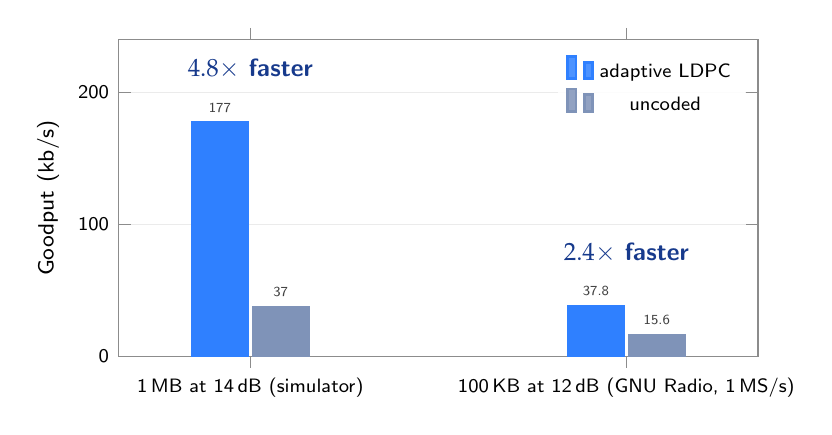
\begin{tikzpicture}
\begin{axis}[wlbar,width=0.8\linewidth,height=56mm,ymin=0,ymax=240,bar width=20pt,
  symbolic x coords={sim,grc},xtick=data,xticklabels={{1\,MB at 14\,dB (simulator)},{100\,KB at 12\,dB (GNU Radio, 1\,MS/s)}},
  ylabel={Goodput (kb/s)},legend style={at={(0.98,0.97)},anchor=north east},enlarge x limits=0.35]
\addplot[fill=wlblue,draw=wlblue] coordinates {(sim,177)(grc,37.8)};
\addplot[fill=wlsteel,draw=wlsteel] coordinates {(sim,37)(grc,15.6)};
\legend{adaptive LDPC,uncoded}
\node[font=\sffamily\bfseries\small,text=wldeep] at (axis cs:sim,218) {$4.8\times$ faster};
\node[font=\sffamily\bfseries\small,text=wldeep] at (axis cs:grc,78) {$2.4\times$ faster};
\end{axis}
\end{tikzpicture}
\caption{End-to-end goodput with adaptive LDPC and without coding.}\label{fig:codinggain}
\end{figure}

\section{TD-CDMA against spread ALOHA}\label{sec:vsaloha}
Both medium-access schemes were run on the same simulated air (\cref{fig:mac,tab:mac}). The decisive
scenario is the first: four stations each send \SI{100}{KB} to the next, all at once, and every station
hears its own transmitter \SI{25}{dB} above the others, as on the ANTSDRs. TD-CDMA moved
\SIrange{173}{181}{kb/s} in total with 6--24 retransmissions; spread ALOHA moved only
\SIrange{53}{58}{kb/s} and needed 755--900 retransmissions, because every frame that arrived while its
receiver was transmitting was lost. Only on idealised radios that can receive while they transmit
(self-leak \SI{3}{dB}) does ALOHA win, with \SIrange{294}{321}{kb/s}: that is CDMA doing what it was made
for, on radios we do not have.

\begin{figure}[htbp]
\centering
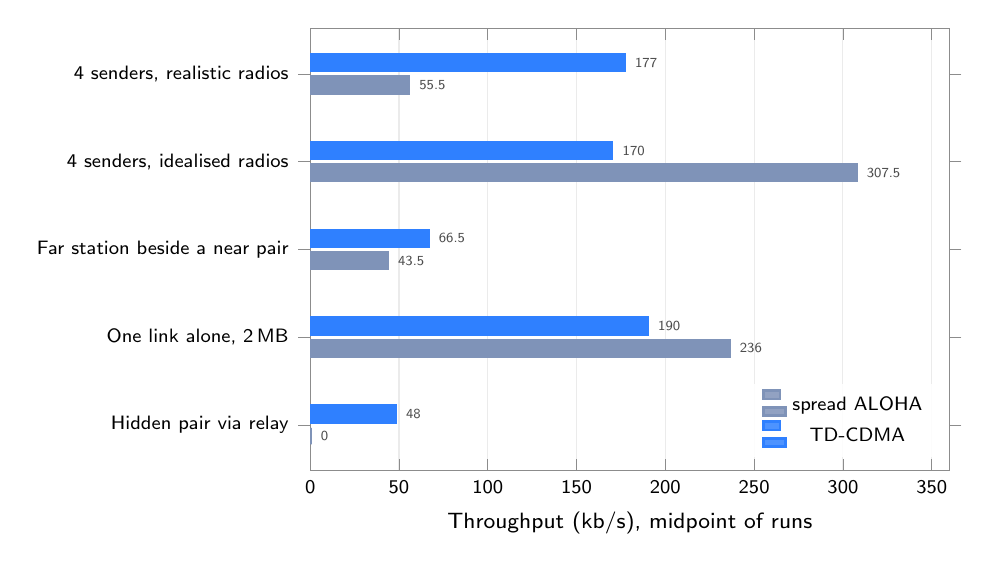
\begin{tikzpicture}
\begin{axis}[wl,xbar,width=0.8\linewidth,height=72mm,xmin=0,xmax=360,bar width=6pt,
  symbolic y coords={hid,one,far,ideal,real},
  ytick=data,yticklabels={Hidden pair via relay,{One link alone, 2\,MB},Far station beside a near pair,{4 senders, idealised radios},{4 senders, realistic radios}},xlabel={Throughput (kb/s), midpoint of runs},xmajorgrids,ymajorgrids=false,
  legend style={at={(0.98,0.03)},anchor=south east},
  nodes near coords,every node near coord/.append style={font=\sffamily\tiny,text=black!70},enlarge y limits=0.13]
\addplot[fill=wlsteel,draw=wlsteel] coordinates {(0,hid)(236,one)(43.5,far)(307.5,ideal)(55.5,real)};
\addplot[fill=wlblue,draw=wlblue] coordinates {(48,hid)(190,one)(66.5,far)(170,ideal)(177,real)};
\legend{spread ALOHA,TD-CDMA}
\end{axis}
\end{tikzpicture}
\caption{TD-CDMA against spread ALOHA on the simulated air. With realistic (self-deafening) radios
TD-CDMA carries three times as much; a hidden pair is reachable only through a TD-CDMA relay.}\label{fig:mac}
\end{figure}

\begin{table}[htbp]
\centering\small
\caption{TD-CDMA and spread ALOHA on the same simulated air.}\label{tab:mac}
\begin{tabularx}{\linewidth}{@{}L>{\raggedright\arraybackslash}p{38mm}>{\raggedright\arraybackslash}p{38mm}@{}}
\toprule
\textbf{Scenario} & \textbf{TD-CDMA} & \textbf{Spread ALOHA}\\
\midrule
4 senders at once, own transmitter 25\,dB above others & \textbf{173--181\,kb/s}, 6--24 resends & 53--58\,kb/s, 755--900 resends\\
4 senders, idealised radios (self-leak 3\,dB) & 160--180\,kb/s, 6--10 resends & \textbf{294--321\,kb/s}, 14--38 resends\\
Near--far, power control off: far station ($-6$\,dB) to a receiver beside a near pair ($+20$\,dB) & far station \textbf{65--68\,kb/s}, 0 resends & far station 43--44\,kb/s, 16 resends\\
One \SI{2}{MB} transfer, \SI{28}{dB} & 190\,kb/s & \textbf{236\,kb/s}\\
Two stations out of each other's range & via relay, \textbf{45--51\,kb/s} & not reachable\\
\bottomrule
\end{tabularx}
\end{table}

TD-CDMA is also fair by construction: every sender gets the same airtime, so the rates of concurrent
senders differ only by their links' rungs (slowest to fastest ratio 0.69--0.82), whereas under ALOHA
the shares depend on who collides with whom.

\section{Near--far problem and power control}
Under spread ALOHA we measured the near--far problem and the effect of power control
(\cref{fig:nearfar}). Alice, Carol and Dave stood together (paths \SI{24}{dB} stronger than to Bob) while
Alice sent a long file to Carol and Bob sent \SI{40}{KB} to Dave. Without power control, Bob's file was
never delivered; with it, Alice backed off by 16--\SI{20}{dB} and Bob's file arrived in 4.6--\SI{9.1}{s}.
Where no station is much nearer than the others, power control cost no speed: in the GNU Radio
channel simulation three simultaneous \SI{150}{KB} transfers took 54.1--\SI{58.1}{s} with it against
64.9--\SI{66.4}{s} before.

\begin{figure}[htbp]
\centering
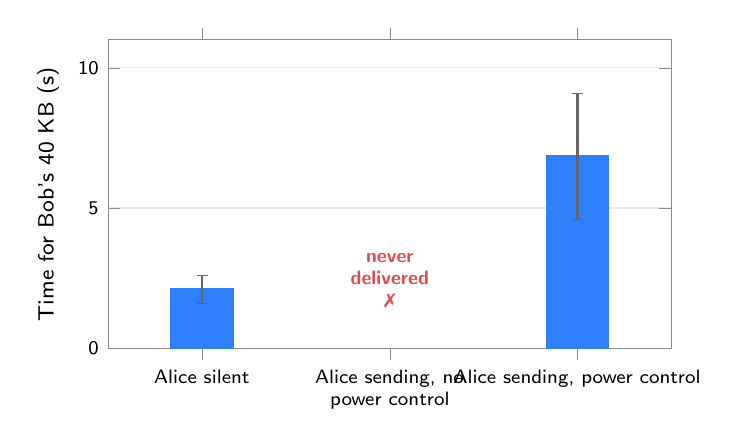
\begin{tikzpicture}
\begin{axis}[wl,ybar,width=0.72\linewidth,height=55mm,ymin=0,ymax=11,bar width=22pt,
  symbolic x coords={silent,off,on},
  xtick={silent,off,on},xticklabels={Alice silent,{Alice sending, no power control},{Alice sending, power control}},x tick label style={text width=32mm,align=center},ylabel={Time for Bob's 40 KB (s)},
  ymajorgrids,xmajorgrids=false,enlarge x limits=0.25]
\addplot[fill=wlblue,draw=wlblue,error bars/.cd,y dir=both,y explicit,error bar style={line width=0.9pt,black!60}]
  coordinates {(silent,2.1) +- (0,0.5) (on,6.85) +- (0,2.25)};
\node[font=\sffamily\bfseries\scriptsize,text=wlcoral,align=center] at (axis cs:off,2.4) {never\\delivered\\\ding{55}};
\end{axis}
\end{tikzpicture}
\caption{Near--far problem under spread ALOHA: Bob's 40\,KB transfer to Dave while Alice, beside Dave,
sends to Carol (bars: midpoint, whiskers: range of four runs).}\label{fig:nearfar}
\end{figure}

\section{Robustness of TD-CDMA}
The edge-case suite runs 17 scenarios on the simulated air in which every receiver's sample counter
starts at a random value and every link has a random delay of up to \SI{100}{\micro s}, so nothing works unless
the offsets are measured. The simulated air records every moment at which two stations transmit while a
third hears both; once a network has formed, this never happened. \Cref{tab:edge} summarises the
results (93 of 93 checks).

\begin{table}[htbp]
\centering\small
\caption{Selected TD-CDMA edge cases on the simulated air.}\label{tab:edge}
\begin{tabularx}{\linewidth}{@{}>{\raggedright\arraybackslash}p{50mm}L@{}}
\toprule
\textbf{Scenario} & \textbf{Result}\\
\midrule
Start orders; four switched on at once; two lone networks meeting & One network every time; four together led by station 1 after 1.4--\SI{2.3}{s}; networks merge under the lower address\\
Station joins and lead leaves during a \SI{300}{KB} transfer & Delivered intact at 136--\SI{163}{kb/s}; no burst late\\
Lead's application closed mid-transfer, then restarted & Successor took over after 0.3--\SI{1.0}{s}; transfer continued; old lead returned as a member\\
Clocks at $+25$, $-25$, $+10$\,ppm for 10 minutes & All 299 messages delivered; $D$ did not move; clock ratios measured within \SI{0.1}{ppm}\\
Six TX underruns and lost RX buffers; a station that cannot hear itself & Both transfers delivered; every jump of $D$ re-measured; the deaf station steered by the others' reports\\
\EsNo\ \SI{5}{dB}; bursty interference \SI{3}{dB} below the signal 25\,\% of the time & Network forms and delivers at \SI{5}{dB}; 117--\SI{138}{kb/s} under interference; no false takeover\\
A station misses every plan announcement (16 changes) & It holds its slot instead of following a stale plan; never overlaps anyone\\
A station stops hearing the lead for \SI{4}{s} & No takeover; it keeps time by the plan another member repeats; transfer continues\\
Group message with a member out of range & Relayed copy for the far member, acknowledgements from both\\
UNO: player away and back; host away & Game pauses and resumes; next player hosts, hands kept\\
\bottomrule
\end{tabularx}
\end{table}

\section{The real flowgraph with emulated ANTSDRs}\label{sec:fakeres}
The strongest evidence before the hardware sessions is the full application running on the unchanged
\code{cdma\_phy.grc}, one process per station, with only the radio blocks emulated (\cref{tab:fake}). The
test PC had two cores, so the air ran at $0.4\times$ real time; 55 of 58 checks passed. The three failures
are one scenario, real-time operation of two stations on the two-core PC, which ran out of CPU (358 TX
underruns and 124 lost RX buffers). Even there no burst was late and no slots overlapped.

\begin{table}[htbp]
\centering\small
\caption{TD-CDMA on GNU Radio with emulated ANTSDRs (GNU Radio 3.10.9, air at $0.4\times$ real time).}\label{tab:fake}
\begin{tabularx}{\linewidth}{@{}>{\raggedright\arraybackslash}p{55mm}L@{}}
\toprule
\textbf{Scenario} & \textbf{Result}\\
\midrule
Start orders; radios switched on together; two lone stations meet & One network every time; led by station 1 after \SI{4.8}{s}; lone networks merged in \SI{1.5}{s}\\
Three \SI{60}{KB} files at once on three links, then a group message & All intact (92, 72 and \SI{51}{kb/s}); group message reached both\\
Lead's process killed mid-transfer & Station 2 took over after \SI{0.71}{s}; transfer continued at \SI{150}{kb/s}, intact\\
Clocks at $+25$, $-25$, $+10$\,ppm & 80 of 80 messages; followers measured $-50.0$ and \SI{-15.0}{ppm}\\
Hidden station, station 2 relays & One network; \SI{40}{KB} from 1 to 3 through 2 at \SI{43}{kb/s}, intact\\
\EsNo\ \SI{10}{dB}; interference 20\,\% of the time & File at \SI{53}{kb/s}; \SI{111}{kb/s} under interference; no false takeover\\
Race and UNO over the slots & 16 of 16 UNO moves seen by both other players\\
\rowcolor{wlcoralpale}Real time, two stations, 2-core PC & \textbf{Failed}: CPU-bound (underruns, lost buffers); still no overlap\\
\bottomrule
\end{tabularx}
\end{table}

\section{Application performance}
\Cref{fig:uno} shows how long a UNO move takes to appear on every screen, and \cref{tab:race} the race
update statistics, both under TD-CDMA in the simulator at \SI{25}{dB}. The move latency grows with the
number of stations because each view waits for its host's slot and each cycle has more slots. Delivery
times for chat messages of every size were shown in \cref{fig:delivery}.

\begin{figure}[htbp]
\centering
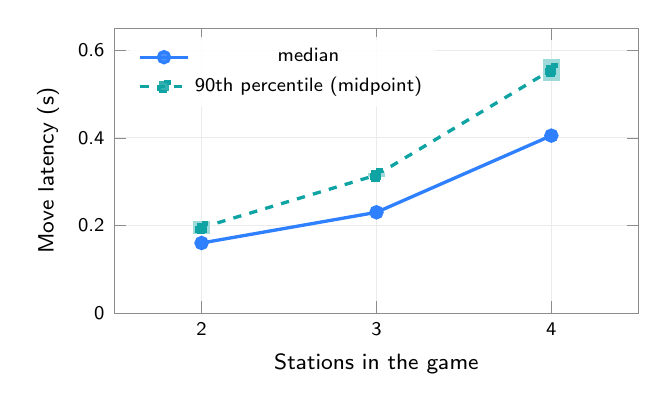
\begin{tikzpicture}
\begin{axis}[wl,width=0.68\linewidth,height=52mm,xmin=1.5,xmax=4.5,ymin=0,ymax=0.65,xtick={2,3,4},
  xlabel={Stations in the game},ylabel={Move latency (s)},legend style={at={(0.03,0.97)},anchor=north west}]
\addplot[wlblue,mark=*,mark size=2pt,line width=1.2pt] coordinates {(2,0.16)(3,0.23)(4,0.405)};
\addlegendentry{median}
\addplot[wlteal,mark=square*,mark size=1.8pt,line width=1.2pt,dashed] coordinates {(2,0.195)(3,0.315)(4,0.555)};
\addlegendentry{90th percentile (midpoint)}
\addplot[wlteal!40,line width=6pt,mark=none,forget plot] coordinates {(2,0.18)(2,0.21)};
\addplot[wlteal!40,line width=6pt,mark=none,forget plot] coordinates {(3,0.31)(3,0.32)};
\addplot[wlteal!40,line width=6pt,mark=none,forget plot] coordinates {(4,0.53)(4,0.58)};
\end{axis}
\end{tikzpicture}
\caption{UNO: time from a move until every screen shows it (shaded: range of the 90th percentile over runs).}\label{fig:uno}
\end{figure}

\begin{table}[htbp]
\centering\small
\caption{Gold Code GP race traffic under TD-CDMA (simulator).}\label{tab:race}
\begin{tabular}{@{}lccc@{}}
\toprule
 & \textbf{2 stations} & \textbf{3 stations} & \textbf{4 stations}\\
\midrule
Updates heard per car per second & 10.0 & 6.1--6.45 & 3.5--3.7\\
Median age of a state when heard & 0.06--\SI{0.08}{s} & 0.07--\SI{0.12}{s} & 0.10--\SI{0.17}{s}\\
Packets lost, events missed, duplicates shown & none & none & none\\
\bottomrule
\end{tabular}
\end{table}

With three and four stations the update rate in the simulator is limited by the PC simulating every
receiver, not by the slots; on hardware every car is heard once per cycle, ten times a second while no
file transfer stretches the cycle.

\section{Computational load}\label{sec:cpu}
Receiver CPU is the binding constraint of the current implementation (\cref{fig:cpu}). Measured with
GNU Radio and emulated ANTSDRs on a \SI{2.8}{GHz} Xeon, a station needs about 1.1 cores per second of air
when idle, 1.2 when sending and 2.1 when receiving at \SI{153}{kb/s}. Of the 2.1 cores, 1.6 are Python
running under a single interpreter lock: the despreader's search and tracking, the link layer, and the
combiner, despreader and LDPC blocks.

\begin{figure}[htbp]
\centering
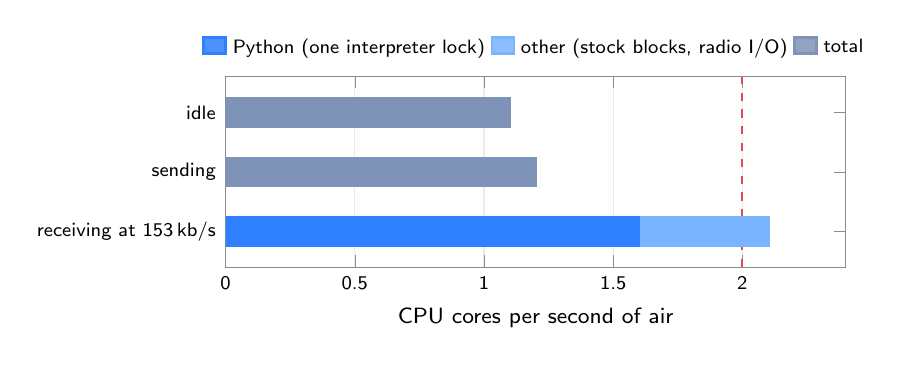
\begin{tikzpicture}
\begin{axis}[wl,xbar stacked,width=0.78\linewidth,height=40mm,xmin=0,xmax=2.4,bar width=10pt,
  symbolic y coords={rx,tx,idle},ytick=data,yticklabels={receiving at 153\,kb/s,sending,idle},xlabel={CPU cores per second of air},
  legend style={at={(0.5,1.04)},anchor=south,legend columns=3},xmajorgrids,ymajorgrids=false,enlarge y limits=0.3]
\addplot[fill=wlblue,draw=wlblue] coordinates {(1.6,rx)(0,tx)(0,idle)};
\addplot[fill=wlsky,draw=wlsky] coordinates {(0.5,rx)(0,tx)(0,idle)};
\addplot[fill=wlsteel,draw=wlsteel] coordinates {(0,rx)(1.2,tx)(1.1,idle)};
\legend{Python (one interpreter lock),{other (stock blocks, radio I/O)},total}
\draw[wlcoral,dashed,line width=0.8pt] (rel axis cs:0.8333,0) -- (rel axis cs:0.8333,1);
\end{axis}
\end{tikzpicture}
\caption{CPU needed by one station (GNU Radio with emulated ANTSDRs, 2.8\,GHz Xeon). The dashed line
marks the two cores of the test PC.}\label{fig:cpu}
\end{figure}

\section{Requirement compliance}
\Cref{tab:compliance} summarises how the final system meets the brief.

\begin{table}[htbp]
\centering\small
\caption{Requirement compliance.}\label{tab:compliance}
\begin{tabularx}{\linewidth}{@{}>{\bfseries\raggedright\arraybackslash}p{42mm}Lc@{}}
\toprule
Requirement & Evidence & Status\\
\midrule
Two-way link over SDRs & 2--4 stations, any pair, both directions; flowgraph with gr-iio blocks & \yes\\
Digital modulation & BPSK, QPSK, 16-QAM over DS-CDMA; FER curves, constellations & \yes\\
Unique addressing & Gold code per station + destination byte; traffic for others never despread & \yes\\
ACK mechanism & Selective-repeat ARQ; ACK records in slot headers; group ACKs per member & \yes\\
CRC error detection & CRC-8 header, CRC-32 frame; dropped frames counted on the dashboard & \yes\\
Packetization and reassembly & \num{1009}-byte fragments, up to \num{65535} per message; tested to \SI{10}{MB} & \yes\\
Text, images, audio & Text, WebP photos, Opus voice notes, any file to \SI{64}{MB} & \yes\\
Application & Chat, UNO and real-time race & \yes\\
Bonus: encryption, priority, dashboard & AES-256-GCM; four priority classes; live radio dashboard & \yes\\
Beyond the brief & LDPC + AMC, power control, TD-CDMA, relaying, emulated-ANTSDR testing & $\bigstar$\\
\bottomrule
\end{tabularx}
\end{table}

%% =====================================================================
\chapter{Challenges, Limitations and Future Work}\label{ch:discussion}
%% =====================================================================

\section{Challenges and how they were solved}
\Cref{tab:challenges} lists the main engineering challenges of the project and the solution adopted
for each.

\begin{table}[htbp]
\centering\small
\caption{Engineering challenges and solutions.}\label{tab:challenges}
\begin{tabularx}{\linewidth}{@{}>{\bfseries\raggedright\arraybackslash}p{45mm}L@{}}
\toprule
Challenge & Solution\\
\midrule
Station deaf while transmitting & One transmitter per slot (TD-CDMA); ACKs in the receiver's own slot\\
0.2--\SI{0.6}{s} transmit latency & Bursts scheduled to the chip in radio samples; plan changes announced \SI{1}{s} ahead\\
Near--far problem & One transmitter at a time; closed-loop power control (target \SI{25.5}{dB})\\
Hidden stations & Link tables in every header; one-hop relaying; plan repeated for stations that miss the lead\\
Carrier and clock offsets between radios & Differential detector ($\pm\SI{16}{kHz}$), 96-symbol CFO fit, 2nd-order carrier loop, DLL to \SI{30}{ppm}\\
16-QAM limited to $\approx$\SI{12}{dB} by timing error & Fractional-delay despreading with $1/64$-sample resolution\\
CPU-bound Python receiver & Slot-aware search (3.2$\to$\SI{1.2}{s} per second of air); DSP in a worker thread\\
Clock drift, stream slips, unknown buffering & TX$\to$RX offset $D$ measured from own bursts; quiet probes; timing feedback\\
Low and changing SNR & 5G NR LDPC with adaptive modulation and coding: $4.8\times$ at \SI{14}{dB}\\
Bugs that only the real flowgraph shows & Emulated ANTSDRs running the unchanged flowgraph: nine timing bugs found and fixed\\
\bottomrule
\end{tabularx}
\end{table}

\section{Limitations}
\begin{warnbox}[Real-time operation on the ANTSDRs]
The TD-CDMA system has run on the real flowgraph only with emulated ANTSDRs, at $0.4\times$ real time,
because the test PC has two cores. A receiving station needs about 2.1 cores, so real-time operation
needs a PC with four or more cores, and has still to be demonstrated on the physical radios.
\end{warnbox}

\begin{itemize}
  \item \textbf{Analog front end not modelled.} AGC, IQ imbalance, DC offset, phase noise, multipath, the
        E200's Ethernet jitter and the real self-leak level are outside our simulators. Power control,
        in particular, has run only in simulation and is digital: the transmitter's own noise floor does
        not drop with it.
  \item \textbf{Single path.} There is no RAKE receiver or equaliser. With \SI{0.5}{\micro s} chips,
        indoor delay spreads of tens of nanoseconds mostly stay within one chip, but 16-QAM in a large
        room may suffer.
  \item \textbf{Detection limits the low end.} Coded QPSK $\tfrac12$ would decode at about \SI{1.5}{dB}, but
        the 48-symbol preamble is detected reliably only from about \SI{4}{dB}.
  \item \textbf{Slot latency for mid-size messages.} With three or four stations an idle slot is shorter
        than one full frame, so a message of a few kilobytes waits about \SI{1.4}{s} for its sender's slot to
        grow; relayed transfers start 2--\SI{5}{s} late for the same reason.
  \item \textbf{One hop, four stations, one key.} Relaying is limited to one hop, the flowgraph has five
        code lanes (four stations plus broadcast), and encryption uses one pre-shared key.
  \item \textbf{Throughput ceiling.} About \SI{236}{kb/s} per link under ALOHA and \SI{190}{kb/s} under
        TD-CDMA, limited by the chip rate that Python DSP can sustain.
\end{itemize}

\section{Future work}
\begin{enumerate}
  \item \textbf{C++ blocks for the hot paths.} Porting the despreader's search and tracking, the burst
        combiner and the LDPC decoder to C++ out-of-tree blocks would remove most of the CPU load and
        allow chip rates of around \SI{10}{MS/s}.
  \item \textbf{Incremental redundancy (HARQ type II).} On a decoding failure, send more parity of the same
        codeword (5G redundancy versions 1--3) and combine it with what was received, instead of resending
        the whole frame.
  \item \textbf{A longer preamble} (96 symbols) to gain about \SI{3}{dB} of detection range.
  \item \textbf{A 2--3 finger RAKE receiver} for multipath in large rooms.
  \item \textbf{Adaptive spreading} (31, 63 or 127 chips by measured SNR) to extend range further.
  \item \textbf{Orthogonal codes inside a slot.} Walsh codes under one scrambling code would remove the
        residual interference between the codes of one transmitter (29.4\,dB with two codes), at the cost of
        chip-synchronous bursts and new preambles.
  \item \textbf{Multi-hop relaying, more stations and per-pair keys} (X25519 key exchange in the
        beacons for forward secrecy).
  \item \textbf{Fragments that fit an idle slot}, so that mid-size messages need not wait for a slot to grow.
\end{enumerate}

%% =====================================================================
\chapter{Conclusion}\label{ch:conclusion}
%% =====================================================================
WaveLink Chat meets every requirement of the \CourseCode\ project brief and goes well beyond it. Instead of
a single point-to-point link, we designed and implemented a self-organising radio network of two to
four ANTSDR\,E200 stations, with a physical layer built as a 68-block GNU Radio flowgraph, a link layer
with reliable, prioritised and adaptive delivery, and an application that combines a modern messenger
with two multiplayer games.

The central lesson of the project is that the right design follows from the hardware, not from the
textbook. Spread ALOHA, the most natural CDMA scheme, collapsed on radios that are deaf while they
transmit; measuring this led us to TD-CDMA, which keeps the advantages of codes (physical-layer
addressing, simultaneous transmission to several destinations, processing gain) while giving every
transmission the channel to itself. Keeping time in radio samples, with each station's
transmit-to-receive offset measured from its own bursts, made slots with a \SI{0.5}{ms} guard possible
despite hundreds of milliseconds of software latency. The 5G NR LDPC code with adaptive modulation and
coding operates within about \SI{2}{dB} of capacity on an ideal channel and multiplied the goodput of a
weak link by $4.8$.

Equally important was the verification strategy. A ladder of simulation environments, ending with the
unchanged flowgraph running against emulated ANTSDRs, exposed nine timing bugs that no simpler
simulation could show, and gave us confidence in every layer before the shared hardware was available.
The remaining step, real-time operation on the physical radios, depends mainly on giving each station
enough CPU; the clear path beyond it is to move the signal-processing hot spots into C++ blocks.

%% =====================================================================
%%  References
%% =====================================================================
%% =====================================================================
%%  References (IEEE style)
%% =====================================================================
\renewcommand{\bibname}{References}
\begingroup
\small
\begin{thebibliography}{99}
\addcontentsline{toc}{chapter}{References}
\setlength{\itemsep}{2pt}

\bibitem{brief} \CourseCode\ Course Project (2026), ``Two-way digital communication system using
software defined radios,'' project brief, \CourseName, 2026.

\bibitem{gold1967} R.~Gold, ``Optimal binary sequences for spread spectrum multiplexing,''
\emph{IEEE Trans. Inf. Theory}, vol.~13, no.~4, pp.~619--621, Oct. 1967.

\bibitem{proakis} J.~G. Proakis and M.~Salehi, \emph{Digital Communications}, 5th~ed.
New York, NY, USA: McGraw-Hill, 2008.

\bibitem{sklar} B.~Sklar, \emph{Digital Communications: Fundamentals and Applications}, 2nd~ed.
Upper Saddle River, NJ, USA: Prentice Hall, 2001.

\bibitem{viterbi1995} A.~J. Viterbi, \emph{CDMA: Principles of Spread Spectrum Communication}.
Reading, MA, USA: Addison-Wesley, 1995.

\bibitem{abramson1970} N.~Abramson, ``The ALOHA system---Another alternative for computer
communications,'' in \emph{Proc. AFIPS Fall Joint Computer Conf.}, 1970, pp.~281--285.

\bibitem{ieee80211} \emph{IEEE Standard for Information Technology---Telecommunications and
Information Exchange Between Systems---Local and Metropolitan Area Networks---Specific Requirements,
Part 11: Wireless LAN Medium Access Control (MAC) and Physical Layer (PHY) Specifications},
IEEE Std 802.11-2020, 2021.

\bibitem{gallager1962} R.~G. Gallager, ``Low-density parity-check codes,'' \emph{IRE Trans. Inf.
Theory}, vol.~8, no.~1, pp.~21--28, Jan. 1962.

\bibitem{ts38212} 3GPP, ``NR; Multiplexing and channel coding,'' 3rd Generation Partnership
Project, Tech. Spec. TS~38.212.

\bibitem{richardson2018} T.~Richardson and S.~Kudekar, ``Design of low-density parity check codes
for 5G new radio,'' \emph{IEEE Commun. Mag.}, vol.~56, no.~3, pp.~28--34, Mar. 2018.

\bibitem{hocevar2004} D.~E. Hocevar, ``A reduced complexity decoder architecture via layered
decoding of LDPC codes,'' in \emph{Proc. IEEE Workshop on Signal Processing Systems (SiPS)}, 2004,
pp.~107--112.

\bibitem{chen2002} J.~Chen and M.~P.~C. Fossorier, ``Near optimum universal belief propagation
based decoding of low-density parity check codes,'' \emph{IEEE Trans. Commun.}, vol.~50, no.~3,
pp.~406--414, Mar. 2002.

\bibitem{golay1949} M.~J.~E. Golay, ``Notes on digital coding,'' \emph{Proc. IRE}, vol.~37, no.~6,
p.~657, Jun. 1949.

\bibitem{macwilliams1977} F.~J. MacWilliams and N.~J.~A. Sloane, \emph{The Theory of
Error-Correcting Codes}. Amsterdam, The Netherlands: North-Holland, 1977.

\bibitem{shannon1948} C.~E. Shannon, ``A mathematical theory of communication,'' \emph{Bell Syst.
Tech. J.}, vol.~27, no.~3, pp.~379--423, Jul. 1948.

\bibitem{gardner1993} F.~M. Gardner, ``Interpolation in digital modems---Part~I: Fundamentals,''
\emph{IEEE Trans. Commun.}, vol.~41, no.~3, pp.~501--507, Mar. 1993.

\bibitem{mengali1997} U.~Mengali and A.~N. D'Andrea, \emph{Synchronization Techniques for Digital
Receivers}. New York, NY, USA: Plenum Press, 1997.

\bibitem{gnuradio} GNU Radio Project, ``GNU Radio: the free and open software radio ecosystem.''
[Online]. Available: \url{https://www.gnuradio.org}

\bibitem{antsdr} MicroPhase, ``ANTSDR E200,'' Crowd Supply product page. [Online]. Available:
\url{https://www.crowdsupply.com/microphase-technology/antsdr-e200}

\bibitem{ad9361} Analog Devices, ``AD9361: RF agile transceiver,'' data sheet.

\bibitem{libiio} Analog Devices, ``libiio: library for interfacing with Linux IIO devices,''
documentation and wiki. [Online]. Available: \url{https://wiki.analog.com/resources/tools-software/linux-software/libiio}

\bibitem{sionna} J.~Hoydis, S.~Cammerer, F.~Ait~Aoudia, A.~Vem, N.~Binder, G.~Marcus, and A.~Keller,
``Sionna: An open-source library for next-generation physical layer research,'' arXiv:2203.11854, 2022.

\bibitem{aff3ct} A.~Cassagne, O.~Hartmann, M.~L\'eonardon, K.~He, C.~Leroux, R.~Tajan, O.~Aumage,
D.~Barthou, T.~Tonnellier, V.~Pignoly, B.~Le~Gal, and C.~Jego, ``AFF3CT: A fast forward error
correction toolbox!,'' \emph{SoftwareX}, vol.~10, 2019, Art. no.~100345.

\bibitem{gcm} M.~Dworkin, ``Recommendation for block cipher modes of operation: Galois/Counter
Mode (GCM) and GMAC,'' NIST Special Publication 800-38D, Nov. 2007.

\bibitem{scrypt} C.~Percival and S.~Josefsson, ``The scrypt password-based key derivation
function,'' IETF RFC~7914, Aug. 2016.

\bibitem{opus} J.-M. Valin, K.~Vos, and T.~Terriberry, ``Definition of the Opus audio codec,''
IETF RFC~6716, Sep. 2012.

\bibitem{rappaport} T.~S. Rappaport, \emph{Wireless Communications: Principles and Practice},
2nd~ed. Upper Saddle River, NJ, USA: Prentice Hall, 2002.

\end{thebibliography}
\endgroup
%% =====================================================================
%%  Appendices
%% =====================================================================
\appendix
\addtocontents{toc}{\protect\setcounter{tocdepth}{0}}

\chapter{The PHY Flowgraph as Saved}\label{app:grc}
\Cref{fig:grcrender} is a rendering of the block layout stored in \code{grc/cdma\_phy.grc}, produced
from the file itself by the project's \code{tools/render\_grc.py}. From top to bottom: the parameter
and variable blocks (sample rate, samples per chip, spreading factor, preamble length, roll-off, the
five Gold codes and the three constellation objects); the transmit chain with its five code lanes
converging on the CDMA Burst Combiner, the RRC filter and the PlutoSDR Sink; and the receive chain from
the PlutoSDR Source through the FFT filter and CDMA Despreader to the three soft-decoder branches, the
LDPC Decoder and the CRC check. Embedded Python blocks are drawn in yellow.

\begin{figure}[p]
\centering
\includegraphics[angle=90,width=\textwidth]{figures/grc_render.pdf}
\caption[Layout of the PHY flowgraph file as stored]{Block layout stored in \code{cdma\_phy.grc}, drawn from the file by the project's layout tool (vector graphic: zoom in to read the blocks).}
\label{fig:grcrender}
\end{figure}

\chapter{Running WaveLink}\label{app:run}

\section{Installation}
\noindent Each laboratory PC needs Ubuntu 22.04 or 24.04 with GNU Radio 3.10 or later (which includes \code{grcc}
and the gr-iio PlutoSDR blocks) and NumPy; the \code{cryptography} package is needed only for
encryption. The web server uses only the Python standard library.
\begin{lstlisting}[language=bash]
sudo apt install gnuradio python3-numpy
python3 -c "from gnuradio import iio; print('gr-iio ok')"
pip install cryptography            # only for --key
\end{lstlisting}
The ANTSDR\,E200 boots its Pluto-compatible firmware from QSPI (boot switch) and is reached at
\code{ip:192.168.1.10}; several radios on one switch need different addresses
(\code{fw\_setenv ipaddr\_eth 192.168.1.11}). TX1 and RX1 are used with separate antennas a few
centimetres apart.

\section{Command-line options}
\begin{table}[htbp]
\centering\small
\caption{Main options of \code{python3 -m wavelink run}.}\label{tab:flags}
\begin{tabularx}{\linewidth}{@{}>{\ttfamily\small}p{31mm}>{\ttfamily\small}p{31mm}L@{}}
\toprule
\textrm{\textbf{Option}} & \textrm{\textbf{Default}} & \textbf{Meaning}\\
\midrule
-{}-id, -{}-name & \textrm{--} & Station address (1--4, also its Gold code) and display name\\
-{}-uri & ip:192.168.1.10 & ANTSDR libiio address (\code{fake:} for emulated radios)\\
-{}-mod, -{}-fec & auto, auto & Restrict modulation (bpsk, qpsk, 16qam) or code rate (off, 1/2 \ldots\ 5/6)\\
-{}-mac & tdcdma & Medium access: TD-CDMA or the earlier spread ALOHA\\
-{}-relay & on & Pass on messages for stations that cannot hear each other\\
-{}-key & \textrm{--} & Passphrase for AES-256-GCM encryption\\
-{}-power-control & on & Transmit power control; \code{-{}-pc-target} sets the target (25.5\,dB)\\
-{}-tx-atten, -{}-rx-gain & 10\,dB, 40\,dB & ANTSDR transmit attenuation and receive gain\\
-{}-tx-buffer & 65536 & ANTSDR transmit buffer in samples\\
-{}-freq & 2.5e9 & Carrier frequency (must match on every station)\\
\bottomrule
\end{tabularx}
\end{table}

\section{Simulators}
\begin{lstlisting}[language=bash,basicstyle=\ttfamily\scriptsize]
# numpy channel simulator, four stations on http://localhost:8081 ... 8084
python3 -m wavelink sim --nodes 4
# Alice and Carol out of each other's range: messages relayed through Bob
python3 -m wavelink sim --nodes 3 --cut 1:3
# the flowgraph PHY over a GNU Radio channel model (three stations)
python3 -m wavelink grc-sim --noise 0.05
# emulated ANTSDRs: start the air, then one real station per terminal
python3 -m wavelink fake-air
python3 -m wavelink run --id 1 --name Alice --uri fake: --port 8081
\end{lstlisting}

\chapter{Division of Work}\label{app:work}
% EDIT: adjust this table to the way your team actually divided the work.
\begin{table}[htbp]
\centering\small
\caption{Main responsibilities of the team members.}\label{tab:work}
\begin{tabularx}{\linewidth}{@{}>{\bfseries\raggedright\arraybackslash}p{38mm}L@{}}
\toprule
Member & Responsibility\\
\midrule
\MemberA & PHY signal processing and coding: Gold codes, modem, LDPC and Golay codes, error-rate measurements, hardware gain tuning\\
\MemberB & GNU Radio and hardware: the \code{cdma\_phy.grc} flowgraph and its Embedded Python blocks, ANTSDR set-up, mid-evaluation tools\\
\MemberC & Link layer and medium access: ARQ, adaptive modulation and coding, power control, priority, TD-CDMA time slots, relaying, simulators\\
\MemberD & Application and user interface: messaging, encryption, game center, radio dashboard, demonstration script\\
\bottomrule
\end{tabularx}
\end{table}

\end{document}
